\chapter{面向双界面商用智能卡ECDSA实现的电磁分析方法}\label{chap:search2}{
	确保密码硬件单元物理安全性检测评估结果的准确性和可靠性,高度依赖于所使用的先进、高效的侧信道分析方法。因此,为确保密码硬件单元物理安全性评估体系的准确性、可靠性和前沿性,有必要持续深入研究并发展先进、高效的侧信道分析方法。%DL-SCA是一类强大的侧信道分析方法,但实际应用DL-SCA时还存在DL-SCA量化指标选择不合理、计算量巨大、采集电磁迹消耗的时间长、恢复私钥的理论时间长等问题。
	
	%本文以分析一款双界面商用智能卡为例,开展了面向基于深度学习侧信道分析的数据增强方法应用示例研究,提出了新的预处理技术并应用了\chapref{chap:search1}的方法和基于假设检验的敏感信息泄漏估计方案,有效提升了DL-SCA在双界面商用智能卡分析场景中的技术效果。在缺少双界面商用智能卡产品设计细节、ECDSA实现所使用的防护对策未知的情况下,成功实现了一款具有ECDSA签名功能的双界面商用智能卡的破解。本文首先进行信息泄漏预处理,将DL-SCA的训练阶段计算量减小到$1.727\cdot10^{11}$浮点运算次数,为原来的0.16\%,DL-SCA变得可行。在不改进网络架构的情况下,使用数据增强进行DL-SCA可以将恢复双界面商用智能卡ECDSA签名信息泄漏的真阳性率由91.35\%提升到95.50\%。使用基于假设检验的估计方案后,真阳性率进一步提升到100\%。这使得从理论上讲,在侧信道分析之后使用格方法恢复双界面商用智能卡ECDSA私钥的时间会从超过七百万年减少到12.5年,再进一步减少到400秒,包含采样时间在内的攻击总时间变为4天,深度学习侧信道方法在双界面商用智能卡分析场景中的攻击成本显著降低。
	
	%具体来说,本研究选择DL-SCA作为主体,选取ECDSA中的一次性随机数泄漏作为攻击目标,使用格基规约从一次性随机数泄漏推算私钥。在这个过程中,提出模数转换、去抖动、高斯模糊多种预处理技术及其组合实现特征点(Point of Interest, POI)高效、准确地提取,使用面向基于深度学习侧信道分析的数据增强方法减少对训练数据的依赖,依据ECDSA签名实现本身的特点定制最有助于恢复私钥的估计方法提高格基规约的成功率。最终成功在可接受的时间内恢复了双界面商用智能卡ECDSA私钥。本文的分析思路和技术方法可以应用于其他类型的双界面商用智能卡分析场景中,为开展其他类似密码硬件单元的分析与破解提供可行的思路和真实的案例。
	
		
	本文以分析一款双界面商用智能卡为例,开展了电磁分析方法研究,减少了DL-SCA时间,提高了DL-SCA真阳性率。本研究使用了\yuchuli 技术、\shujuzengqiang、\jiashejianyanguji。在现有实验环境下,成功实现了对型号为J3D081的Java卡的电磁分析,在1天内采集5000条电磁迹、3天内进行电磁迹预处理得到样本数量为十万的数据集、137秒内对数据集中的训练集进行数据增强、1小时内实施DL-SCA恢复敏感信息泄漏。电磁分析后可以从5000条电磁迹对应的的签名中,过滤出119条可以被后续格方法所利用的含有连续4比特敏感信息泄漏的签名,且这119条签名含有的连续4比特敏感信息泄漏都正确。达到了后续使用由敏感信息泄漏恢复私钥的格方法的条件。%在分析双界面商用智能卡的ECDSA实现时,需要将侧信道分析与格方法结合才可能利用当前实验环境在可接受的时间范围内恢复私钥。在实际分析时,电磁迹采样点多导致深度学习模型训练时间长达315天,电磁迹特征点不明显导致运用格方法恢复ECDSA私钥的时间达到约$2\times10^{85}$年,仍然超过可接受的时间范围。本研究提出并使用\yuchuli 预处理技术,以增加3天的预处理时间为代价,将DL-SCA时间由315天减小为8分钟,将运用格方法的时间由约$2\times10^{85}$年减小到约$7\times10^{6}$年。本研究使用\chapref{chap:search1}的面向基于深度学习侧信道分析的通用数据增强方法,以增加2分钟的数据增强时间和1小时的DL-SCA时间为代价,将运用格方法的时间由约$7\times10^{6}$年减小到约12.5年。本研究提出并使用\jiashejianyanguji 方案,将运用格方法的时间由约12.5年减小到400秒。本研究仅用4天就恢复了ECDSA私钥,其分析思路和技术方法可以应用于其他类型的双界面商用智能卡分析场景中,为开展其他类似密码硬件单元的分析与破解提供可行的思路和真实的案例。
	
	\yuchuli 技术通过\poifanwei 技术将特征点范围从五千万缩小到1.8万,接着使用相关系数极值点的时间模板实现特征点提取,执行TVLA后可以检测出泄漏。\yuchuli 技术提取了特征点,完成了电磁迹的预处理,成功构造了用于深度学习的数据集。
	\shujuzengqiang 选择最优的数据增强策略参数对现有数据集中的训练集进行数据增强,使得实际攻击时在不额外采集电磁迹的情况下将DL-SCA的真阳性率由91.35\%提高到95.50\%。
	\jiashejianyanguji 利用格方法攻击目标双界面商用智能卡ECDSA实现的特点(对敏感信息泄漏估计值假阳性敏感,假阴性不敏感),通过使用更严格的标准估计阳性样本。在使用本研究采集的数据、独立进行5次进行深度学习模型的训练和测试、每次使用5000条电磁子迹进行测试、显著水平$\alpha=0.51056$的前提下,真阳性率都达到100\%。
	本研究分析思路和技术方法可以应用于其他类型的双界面商用智能卡分析场景中,为开展其他类似密码硬件单元的分析与破解提供可行的思路和真实的案例。
	
	\secref{sec:vulnerable}介绍了作为本研究攻击目标的双界面商用智能卡ECDSA实现的预备知识,\secref{sec:hardpoint}介绍了攻击智能卡存在的难点,\secref{sec:hardpoint}详细说明了解决现有问题的技术方案,\secref{sec:ecdsaresult}以双界面商用智能卡ECDSA实现为例,汇报了实施面向智能卡电磁分析的技术效果。
	
%	\begin{table}[!h]
%		\bicaption{\enspace 攻击智能卡待解决的问题}{\enspace Nuts to crack in attacking the smart card}
%		\label{tab:problemset}
%		\centering
%		\scriptsize% fontsize
%		%\setlength{\tabcolsep}{4pt}% column separation
%		%\renewcommand{\arraystretch}{1.2}%row space 
%		\begin{tabular}{ll|ll}
%			\hline
%			\multicolumn{2}{c|}{现有问题} & 不解决会造成的后果&本研究的解决方案\\
%			\hline
%			实验条件&示波器采样深度低&攻击所需的电磁迹增加&暂无解决方案\\
%			\hline
%			\multirow{2}{*}{量化指标选择}&准确率等指标不适合本研究&\multirow{2}{*}{分析技术的优化方向错误}&\multirow{2}{*}{使用敏感信息泄漏估计真阳性率}\\
%			&猜测熵等指标难以定义&&\\
%			\hline
%			\multirow{3}{*}{分析技术选择}&缺少计算资源&无法进行DL-SCA&提取特征点,减小计算量\\
%			&依赖大量样本进行训练&增加采集电磁迹的时间开销&使用\chapref{chap:search1}的数据增强方法\\
%			&极大似然估计不适合本研究&增加运用格方法恢复私钥的时间&设定基于假设检验的估计方案\\
%			\hline
%		\end{tabular}
%	\end{table}

	\section{ECDSA攻击预备知识}\label{sec:vulnerable}
	\subsection{智能卡ECDSA签名实现推测}
	
	作为研究目标的智能卡所属的产品家族(Product Family)为J3D081,它是符合ISO7816\citep{ISO/IEC7816}与ISO14443 A\citep{ISO/IEC14443}规范的双界面的Java产品,其JCOP版本是Java Card3.0.1,GlobalPlatform版本是2.2.1。该智能卡使用了SmartMX\citep{p5x}安全微控制器芯片。Roche等\citep{Roche21}对同样使用SmartMX的两款智能卡进行过研究,并对其在ECDSA算法中的数乘实现进行了分析和猜想。因为芯片型号完全相同,我们认为J3D081智能卡与Roche等\citep{Roche21}研究的智能卡中ECDSA中的数乘实现也相同。
	
	Roche等\citep{Roche21}对智能卡中数乘实现进行了分析,依据分析结果对签名操作的数乘算法进行了推测。签名操作的数乘$\nonce\cdot G$应当执行如下步骤进行了计算:
	
	\begin{itemize}
		\item 使用\algorithmref{alg:encodek}将一次性随机数$\nonce$转化为长度为129的编码形式$\left\{\tilde{\nonce}_0,\tilde{\nonce}_1,\dots,\tilde{\nonce}_{128}\right\}$。
		\item 使用\algorithmref{alg:improvesignscalar}计算数乘结果。
	\end{itemize}

	\noindent 其中,\algorithmref{alg:encodek}的输入$\multiplier=\nonce,cl=129$,\algorithmref{alg:improvesignscalar}的输入$\left\{\tilde{\nonce}_0,\tilde{\nonce}_1,\dots,\tilde{\nonce}_{128}\right\}$是\algorithmref{alg:encodek}的输出,$G_1,G_2,G_3,G_4$是不必重复计算的\footnote{这些值在确定椭圆曲线$E$和生成元$G$之后就可以预计算,将计算结果硬编码进外存。每次签名时,将外存的数据载入内存参与运算即可完成签名。因此这些值是不必重复计算的。}椭圆曲线$E$上的点,$G_1=G,G_2=2^{129}\cdot G,G_3=\left(2^{129}+1 \right) \cdot G,G_4=2^{128}\cdot G$,$G$是选定椭圆曲线$E$的同时所选定的生成元。
	
	\begin{breakablealgorithm}
		\caption{窗口大小为2的大数编码算法}\label{alg:encodek}
		\begin{algorithmic}[1]
			\Statex \textbf{输入:} $\multiplier$:被编码的整数
			\Statex \textbf{输入:} $cl$:目标编码的长度
			\Statex \textbf{输出:} $\left\{\tilde{\multiplier}_0,\tilde{\multiplier}_1,\dots,\tilde{\multiplier}_i,\dots, \tilde{\multiplier}_{cl-1}\right\}$:$\multiplier$的长度为$cl$的编码形式
			\State 计算$\multiplier$的二进制表示$\sum\limits_{i=0}^{2cl-1}\multiplier_i2^{2cl-i-1}=\multiplier$
			\For{$i := 0, \dots, cl-1$}
			\State $\tilde \multiplier_i:=2\multiplier_i+\multiplier_{i+cl}$
			\EndFor
			\State \Return $\left\{\tilde{\multiplier}_0,\dots,\tilde{\multiplier}_i,\dots, \tilde{\multiplier}_{cl-1}\right\}$
		\end{algorithmic}
	\end{breakablealgorithm}

	\begin{breakablealgorithm}
		\caption{改进后签名操作的数乘算法}\label{alg:improvesignscalar}
		\begin{algorithmic}[1]
			\Statex \textbf{输入:} $\left\{\tilde{\nonce}_0,\tilde{\nonce}_1,\dots,\tilde{\nonce}_j,\dots, \tilde{\nonce}_{128}\right\}$:一次性随机数$\nonce$的长度为129的编码形式
			\Statex \textbf{输入:} $G_1,G_2,G_3,G_4$:预计算的椭圆曲线$E$上的点
			\Statex \textbf{输出:} $\nonce\cdot G$:基点$G$与一次性随机数$\nonce$数乘的结果
			\State $S:=G_1$
			\For{$j:=1,\dots , 128$}
			\State $S:=2\cdot S$
			\If {$\tilde \nonce_j>0$}
			\State $\leakedmultiplier_j:=\tilde \nonce_j$
			\State $S:=S+G_{\leakedmultiplier_j}$\Comment{$\leakedmultiplier_j$存在泄漏}
			\Else
			\State $\leakedmultiplier_j\stackrel{\$}\gets\{1,1,2,3\}$\Comment{引入随机数}
			\State $Dummy:=S+G_{\leakedmultiplier_j}$\Comment{$\leakedmultiplier_j$存在泄漏}
			\EndIf
			\EndFor
			\If {$\tilde \nonce_0=0$}
			\State $S:=S-G_4$
			\Else
			\State $Dummy:=S-G_4$
			\EndIf
			\State \Return $S$
		\end{algorithmic}
	\end{breakablealgorithm}
	\subsection{随机数部分泄漏的请况下基于格的ECDSA攻击}\label{subs:infoforlattice}
	
	有大量工作\citep{Howgrave-Graham01,Nguyen02,Nguyen03,Hlavac06,Brumley11,Mulder14,Benger14,Goudarzi16,Fan16,Ryan19,Jancar20,Moghimi20,Weiser20,Micheli20}研究了在随机数泄漏少量比特的情况下攻击ECDSA方案,它们的主要思想是利用签名中的随机数的泄漏构造扩展隐藏数问题\citep{Boneh96}的方程并使用格基规约求解。
	
	在本研究中,为了恢复私钥,需要使用格方法从一次性随机数$\nonce$的泄漏求解私钥$\sk$。但是格方法本身不在本文研究范围内,因此只做大致描述。
	
	\begin{figure}[!htb]
		\centering
		\begin{tikzpicture}[node distance=20pt]
			\node[draw, rounded corners,align=center]  (start)  {运算开始};
			\node[draw, trapezium, trapezium left angle=70, trapezium right angle=110,below=of start,align=center](inputleak){输入:用于构造方程的签名及其泄漏};
			\node[draw, below=of inputleak,align=center] (constructequ)  {构造方程};
			\node[draw, below=of constructequ,align=center] (solve)  {使用格基规约算法求解(近似)最短向量};
			\node[draw, below=of solve,align=center] (calcd)  {根据(近似)最短向量求解私钥$\hat \sk$};
			\node[draw, diamond, aspect=2, below=of calcd,align=center]     (chkd)  {$\hat \sk\cdot G=\pk$?};
				
			\node[draw, trapezium, trapezium left angle=70, trapezium right angle=110,align=center]at ([xshift=-40pt,yshift=-35pt]chkd.south west)(success){输出:"求解成功",$\sk=\hat \sk$};
			\node[draw, trapezium, trapezium left angle=70, trapezium right angle=110,align=center]at ([xshift=40pt,yshift=-35pt]chkd.south east)(fail){输出:"求解失败"};
			\node[draw, rounded corners, below=50pt of chkd,align=center]  (end) {运算结束};
				
			\draw[->] (chkd) -|node[midway,very near start,above] {是} (success);
			\draw[->] (chkd) -|node[midway,very near start,above] {否} (fail);
				
			\draw[->] (success) |- (end);
			\draw[->] (fail) |- (end);
			\graph{
				(start)->(inputleak)->(constructequ)->(solve)->(calcd) -> (chkd);
			};
		\end{tikzpicture}
		\bicaption{\enspace 利用随机数部分泄漏使用基于格的ECDSA攻击流程图}{\enspace Flowchart of Lattice-based ECDSA Attacks with Partial Knowledge of the Nonces}
		\label{fig:solver}	
	\end{figure}
	
	运用一次格方法从一次性随机数$\nonce$的泄漏求解私钥$\sk$的过程如\figureref{fig:solver}所示。它首先依据输入构造方程,其次调用格基规约算法求解近似最短向量,然后将近似最短向量视为最短向量以计算出私钥,接着通过公钥对私钥进行验证,最后输出验证结果。之所以需要验证是因为有多种原因会导致求解出错误的私钥。运用一次格方法是伯努利实验,它有一定的失败概率。但是在实际中,运用格方法次数的唯一限制因素是攻击者提供的用于攻击的时间。在攻击时间内,攻击者可以尝试多次运用格方法,直到恢复私钥为止。在这种情况下,只论成功率的大小已经意义不大,因为从理论上讲只要提供足够长的攻击时间,就一定能恢复私钥。%假如运用一次格方法的成功概率固定,且每次运用格方法是否成功互相独立,那么攻击者运用格方法的次数应当服从二项分布。
	
	运用一次格方法的主要时间开销来自于执行其中的格基规约算法。当前的格基规约算法是多项式时间复杂度的近似算法,它有三方面的使用限制:
	
	\begin{enumerate}
		\item 格上的方程应当合理且信息量充足,否则求解失败;
		\item 格上的方程不能含有错误,否则求解失败;
		\item 即使格上的方程合理、信息量充足且不含错误,也可能求解失败。
	\end{enumerate}
	
	如果格上的方程信息量不充足,那么方程欠定,会有无穷多种可行解,因此无法找到所需要的正解,求解失败。如果方程含有错误,会导致运算过程出错,求解失败。在格上的方程信息量充足且不含错误的情况下,因为当前的格基规约算法是近似算法,本身就可能导致计算出的近似解不是正解,求解失败。方程不合理会导致算法执行过程中更可能做出错误的近似,计算出的近似解有更大的可能不是正解,求解失败。
	
	%不失一般性地,不妨假设在侧信道攻击之后仍然存在某些信息泄漏没有恢复\footnote{通常来说,侧信道攻击要求恢复每一处信息泄漏,因为即使存在偶然误差也可以通过平均的方法加以控制。但是对于ECDSA来说,一次性随机数互相独立、一次性随机数每个比特也互相独立,无法使用平均的方法控制随机误差。本研究使用的格方法在仅恢复特定的一部分信息泄漏的情况下依然可以恢复私钥,因此本研究不恢复每一处信息泄漏}。
	本研究在侧信道分析之后会尝试多次运用格方法\footnote{格方法通常是指通过解决格问题来攻击密码系统,而在实践中,可能需要多次尝试和调整参数才能成功恢复私钥},直到成功恢复私钥:
	
	\begin{enumerate}
		\item 枚举每条签名,如果从对应的电磁迹中恢复的敏感信息泄漏估计值$\hat{\tilde \nonce}_j,j=0,1,\dots,128$为0的次序中有连续4位的情况,那么记录这连续4位(如果有多个连续4位的情况,记录一个即可)的位置以及值\footnote{如果$\exists 0\le k<30-4,\hat{\nonce}^{(i)}_k=\hat{\nonce}^{(i)}_{k+1}=\hat{\nonce}^{(i)}_{k+2}=\hat{\nonce}^{(i)}_{k+3},i=0,1,\dots,T_a-1$,那么记录数据对$(i,k)$并同时记录第$i$条签名。},否则排除该签名(不用于后续攻击);
		\item \textbf{随机}选择75条保留下来的签名(如果保留下来的签名不足75条,那么无法求解,需要采集更多电磁迹加以解决);
		\item 利用这些签名的签名消息$hsh=H(m_0)$、签名$(r,s)$、连续4位的被恢复的一次性随机数比特泄漏所在位置以及值、椭圆曲线的阶$q$,构造格上的方程;
		\item 调用格基规约算法BKZ\citep{Schnorr91}进行格基规约,利用近似解求解私钥;
		\item 使用公钥验证私钥,如果验证成功返回私钥,如果验证失败返回第2步。
	\end{enumerate}

	\subsection{符号表示}\label{subs:ecdsasymbol}
	%本研究不区分“估计”和“预测”两个概念。前者用于从假设检验的角度进行理论分析,后者用于描述实践中依据深度学习网络输出的概率向量推断敏感信息泄漏最可能的值的过程。
	本研究严格区分“预测”和“估计”两个概念。前者用于描述深度学习网络输出概率向量的过程,后者用于描述使用数理统计的方法判定是否接受与一个变量的值有关的某种假设。
	
	本研究严格区分这几个概念:敏感信息泄漏、敏感信息泄漏值、敏感信息泄漏估计、敏感信息泄漏估计值。它们的关系如\figureref{fig:leakageill}所示。
	
	\begin{figure}[!h]
		\begin{center}
			\begin{tikzpicture}[node distance=40pt, auto]
				\tikzstyle{obj} = [draw, rounded corners,align=center]
				\tikzstyle{var} = [rectangle, draw,text centered]
				
				\node[var] (leakage) {敏感信息泄漏};
				\node[obj,right=85pt of leakage] (leakageobj) {敏感信息泄漏值};
				\node[var,below= of leakage] (trace) {信息泄漏};
				\node[obj,below= of leakageobj] (traceobj) {迹};
				\node[obj,below= of traceobj] (leakageprobobj) {敏感信息泄漏概率向量};
				\node[obj,below= of leakageprobobj] (leakageestimateobj) {敏感信息泄漏估计值};
				\node[var]at (trace |- leakageestimateobj) (leakageestimate) {敏感信息泄漏估计};
				%		\node[var,below= of leakageestimate] (okleakageestimate) {可利用的敏感信息泄漏估计};
				%		\node[obj,below= of leakageestimateobj] (okleakageestimateobj) {可利用的敏感信息泄漏估计值};
				%		\node[var,below= of okleakageestimate] (usedleakageestimate) {被利用的敏感信息泄漏估计};
				%		\node[obj,below= of okleakageestimateobj] (usedleakageestimateobj) {被利用的敏感信息泄漏估计值};
				
				\draw[dashed] (-60pt,50pt) rectangle (60pt,-200pt);
				\node at (0,40pt) {随机变量};
				
				\draw[dashed] (102pt,50pt) rectangle (390pt,-200pt);
				\node at (246pt,40pt) {样本值(评估者可以得到的信息)};
				
				\draw[dash dot] (105pt,-40pt) rectangle (387pt,-195pt);
				\node at (320pt,-188pt) {攻击者可以得到的信息};
				
				\draw[dash dot] (105pt,20pt) rectangle (387pt,-20pt);
				\node at (320pt,0pt) {攻击者期望得到的信息};
				
				\draw[dashed, -stealth] (trace.south) -- (leakageestimate.north) node[midway, right] {分析技术};
				
				\graph{
					(leakage)->["部分嵌入"](trace);
					(leakage)->["实例化"](leakageobj);
					(trace)->["实例化",pos=0.4](traceobj);
					(leakageestimate)->["实例化"](leakageestimateobj);
					%(okleakageestimate)->["实例化"](okleakageestimateobj);
					%(usedleakageestimate)->["实例化"](usedleakageestimateobj);
					(traceobj)->["(使用DL-SCA)提取并预测"](leakageprobobj)->["(使用基于假设检验的)估计"](leakageestimateobj);
					%(leakageestimate)->["部分可用于格方法"](okleakageestimate)->["部分实际被用于格方法"](usedleakageestimate);
				};
			\end{tikzpicture}
			\bicaption{\enspace 信息泄漏相关概念示意图}{\enspace Schematic diagram of concepts related to information leakage}
			\label{fig:leakageill}
		\end{center}
	\end{figure}
	
	在本研究中每条电磁迹,对应的签名操作所使用的一次性随机数记为$\nonce$。$\nonce$是敏感信息但没有直接泄漏,$\nonce$通过它的编码形式$\left\{\tilde{\nonce}_0,\tilde{\nonce}_1,\dots,\tilde{\nonce}_{128}\right\}$在\algorithmref{alg:improvesignscalar}执行过程中产生泄漏。因为一次性随机数$\nonce$、\algorithmref{alg:encodek}中的$\tilde\nonce_j,j=0,1,2,\dots128$和\algorithmref{alg:improvesignscalar}中的$\nonce_j,j=0,1,2,\dots257$存在等价关系,本研究将这三个变量都称为敏感信息泄漏。

	敏感信息泄漏的值就是敏感信息泄漏值,他们的关系类似于随机变量和随机变量的样本值。每有一条签名,敏感信息泄漏就有一个值。令第$i$条签名对应的敏感信息泄漏值用符号$\nonce^{(i)}$、$\nonce^{(i)}_j,j=0,1,2,\dots257$和$\tilde{\nonce}^{(i)}_j,j=0,1,2,\dots128$表示。

	攻击者无法直接得到敏感信息泄漏值,只能利用所获得的迹,使用某些具体的分析技术(对本研究而言,指的是DL-SCA、数据增强、基于假设检验的估计方案)来获取与敏感信息泄漏值尽可能一致的结果。攻击者获得的这个结果就称为敏感信息泄漏估计值。对于$\nonce^{(i)}$、$\nonce^{(i)}_j,j=0,1,2,\dots257$和$\tilde{\nonce}^{(i)}_j,j=0,1,2,\dots128$,对应的敏感信息泄漏估计值分别用$\hat\nonce^{(i)}$、$\hat\nonce^{(i)}_j,j=0,1,2,\dots257$和$\hat{\tilde\nonce}^{(i)}_j,j=0,1,2,\dots128$表示。
	
	敏感信息泄漏估计值也可以被视为是某种随机变量的样本值。本文将这种随机变量称为敏感信息泄漏估计,$\hat\nonce$、$\hat\nonce_j,j=0,1,2,\dots257$和$\hat{\tilde\nonce}_j,j=0,1,2,\dots128$都是敏感信息泄漏估计。
	
	在\figureref{fig:leakageill}中,“实例化”指的是对随机变量进行采样得到样本值。“部分嵌入”指的是在\algorithmref{alg:improvesignscalar}运算过程中,不是所有的敏感信息$\tilde \nonce^{(i)}_j,i=0,1,\dots T_a,j=0,1,\dots,128$都存在泄漏(因为在某些迭代中,会执行代码第8、9行的分支,而不执行第5、6行的分支)。“分析技术”指的是攻击者可以尝试尽可能多已有技术进行侧信道分析。“提取并预测”指的是使用DL-SCA从电磁迹中得到敏感信息泄漏每种取值对应的概率。“估计”指的是依据概率向量,使用基于假设检验的估计方法对敏感信息泄漏做出最有助于恢复私钥的\footnote{通常来说,会依据极大似然原理做出极大似然的估计。极大似然估计只是使用数理统计估计的一种特殊情况。极大似然的估计反而会导致恢复私钥的时间更长。}估计。
	
	对于攻击者而言,他的目标是找到合适的分析技术,使得敏感信息泄漏估计最有助于恢复私钥\footnote{仅就针对恢复ECDSA私钥而言,最准确(the most accurate)的敏感信息泄漏估计方法不是最有助于恢复私钥的估计方法。},这样一来就能保证后续使用格方法进行攻击时攻击总时间尽可能短。但是在实际侧信道分析中,完全一致难以实现。因此如何选取合理的指标量化评价这种“有助于恢复私钥”的程度、如何选取具体的分析技术使得指标达到最优是一个亟待解决的问题。本研究以针对攻击双界面商用智能卡ECDSA私钥为例,来说明针对具体的问题如何选取合理的量化指标、如何选取合理的分析技术。
	
	虽然$\nonce$、$\tilde\nonce_j,j=0,1,2,\dots128$和$\nonce_j,j=0,1,2,\dots257$两两之间都有对应关系,并且它们都是敏感信息泄漏,但是它们有各有侧重。$\nonce$用于帮助理解ECDSA签名操作以及签名操作的数乘结果,$\tilde\nonce_j,j=0,1,2,\dots128$用于帮助理解敏感信息如何产生了泄漏,$\nonce_j,j=0,1,2,\dots257$用于帮助理解侧信道分析与格方法结合时如何恢复ECDSA私钥。
	
	\section{智能卡ECDSA算法实现侧信道分析难点分析}\label{sec:hardpoint}
	为了以双界面商用智能卡ECDSA实现为目标实施DL-SCA,需要针对这两个难点提出解决方案:1.训练时间长。在本文实验条件下,即使深度学习模型仅使用1个训练样本训练1个迭代轮次,也需要10分钟。使用167个样本训练20轮次理论上需要315天。2.真阳性率低。即使进行了预处理,真阳性率也只有91.35\%。
	
	本研究采集数据的参数如\tableref{tab:acquisitionpara}所示。从中可以看到每条电磁迹的采样时间小于一次数乘时间\footnote{这不能通过降低采样率加以解决。当采样率下降,尽管采集时间变长,但是采集的电磁迹难以分析出敏感信息泄漏,反而影响恢复敏感信息泄漏,增加使用格方法恢复私钥时间。},这会使得在采集阶段本应采集到每次签名操作完整的128次迭代的信息泄漏,但是因为采集条件受限,只能采集到每次签名操作的$n_s$次迭代的信息泄漏。经过实验发现,$n_s$的每次签名操作被采集信息泄漏的迭代次数不超过30。为了方便后续分析,假设在当前的采集条件下可以采集到每次签名操作的前30次迭代的信息泄漏,即令$n_s=30$。
	
	\begin{table}[!h]
		\bicaption{\enspace J3D081采集参数}{\enspace Acquisition parameters on J3D081}
		\label{tab:acquisitionpara}
		\centering
		%\footnotesize% fontsize
		%\setlength{\tabcolsep}{4pt}% column separation
		%\renewcommand{\arraystretch}{1.2}%row space 
		\begin{tabular}{ll}                                                               
			\hline   
			采集参数&参数数值\\                                                          
			\hline
			操作 & ECDSA签名\\
			输入 & 固定消息$m$,(随机选择的)固定私钥$\sk$\\
			哈希函数& sha1\citep{FIPS180-4}\\
			操作次数(能量迹条数) & 5000\\
			一次数乘时间 & 40ms\\
			采样率 & 5GHz\\
			每条电磁迹采样时间 & 10ms\\
			每条电磁迹采样点个数 & 50000000\\
			通道 & 电磁\\
			数据大小 & 1TB\\
			采集时间 & 1天\\
			\hline
		\end{tabular}
	\end{table}

	
	本研究从理论证明了运用格方法恢复私钥(直到成功为止)的时间期望的下界会随着敏感信息泄漏估计真阳性率的减小而成指数级增长,推导过程如\propositionref{prop:expotime}所示。\figureref{fig:expotime}展示了敏感信息泄漏估计真阳性率略小于100\%的情况下多次运用格方法恢复私钥(直到成功为止)在理论上的技术效果,其中橙色实线表示恢复实际私钥的时间的期望的下界,蓝色虚线表示使用指数函数可以对下界的下界做一个很好的估计,不同线型的绿色虚线表示攻击所能容忍的不同程度时间消耗(一小时、一天、一个月)。进一步分析可以知道,如果要求运用格方法分别在一个月、一天、一小时内恢复实际私钥,那么通过侧信道分析所恢复敏感信息泄漏估计真阳性率分别需要达到97.12\%、98.22\%、99.27\%。
	
	\begin{figure}[!h]
		\begin{center}
			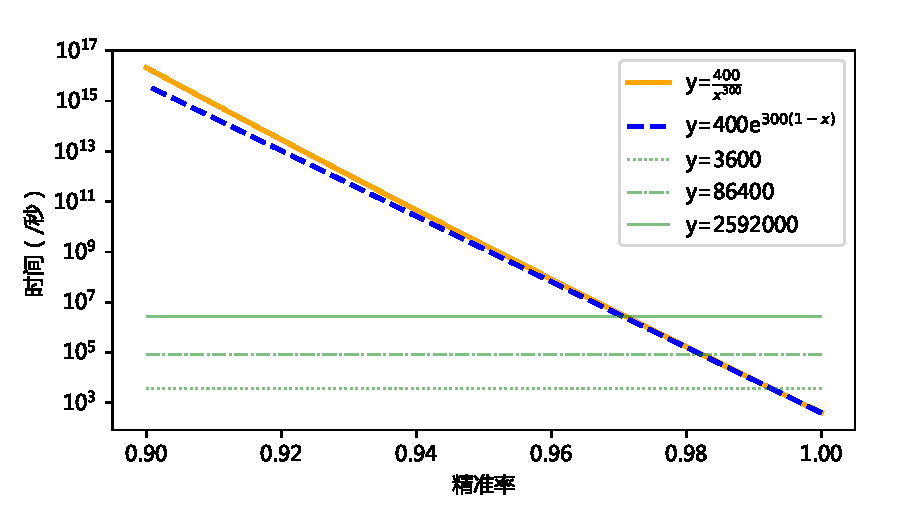
\includegraphics[width=\textwidth]{expotime}
			\bicaption{\enspace 真阳性率对攻击时间期望的影响}{\enspace Impact of true positive rate on the expectation of attack time}
			\label{fig:expotime}
		\end{center}
	\end{figure}

	{\color{\xchange}
		
	\tableref{tab:problemset}汇总了实施对双界面商用智能卡ECDSA实现侧信道分析时,会产生问题的根本原因。采集的电磁迹采样点多会导致执行DL-SCA时间长。采集的电磁迹特征点不明显、敏感信息泄漏估计使用极大似然估计会导致执行DL-SCA真阳性率低。根本原因无法解决,而执行DL-SCA时间长、真阳性率低等问题是可以通过改进DL-SCA的流程来缓解的。%以及相应的解决方案。针对选择量化指标的问题,本研究从理论上说明了敏感信息泄漏估计真阳性率的合理性,并通过实验进行了验证。针对选择合理的分析技术的问题,本研究使用了提出量化、去抖动、高斯模糊多种预处理技术及其组合实现POIs高效、准确地提取,使用面向基于深度学习侧信道分析的数据增强方法减少对训练数据的依赖,依据ECDSA签名实现本身的特点和采集信息泄漏的能力设定了计算敏感信息泄漏估计值的具体方案。
	为了减少执行DL-SCA的时间、提到DL-SCA真阳性率,本研究提出了\yuchuli 技术、\shujuzengqiang、\jiashejianyanguji。
	
	\begin{table}[!h]
		\bicaption{\enspace 导致攻击智能卡存在问题的原因}{\enspace Reasons for the existence of problems in attacking the smart card}
		\label{tab:problemset}
		\centering
		\scriptsize% fontsize
		%\setlength{\tabcolsep}{4pt}% column separation
		%\renewcommand{\arraystretch}{1.2}%row space 
		\begin{tabular}{c|cc}
			\hline
			根本原因&是否导致执行DL-SCA时间长&是否导致DL-SCA真阳性率低\\
			\hline
			采集的电磁迹采样点多&是&/\\
			采集的电磁迹特征点不明显&否&是\\
			敏感信息泄漏估计使用极大似然估计&否&是\\
			\hline
		\end{tabular}
		\tabnote{当电磁迹采样点多时,已经无法在可接受的时间内执行DL-SCA,因此无法获得实际真阳性率。}
	\end{table}

	\section{基于深度学习的电磁分析方法}\label{sec:solution}
	{\color{\xchange}
		
		本研究以深度学习作为主体,引入\yuchuli 技术、\shujuzengqiang 和\jiashejianyanguji 技术,解决了实施对双界面商用智能卡ECDSA实现侧信道分析时存在的具体难点,如\tableref{tab:solution2problem}所示。
		
		\begin{table}[!h]
			\bicaption{\enspace 解决方案与难点的对应关系}{\enspace Solutions to the problems}
			\label{tab:solution2problem}
			\centering
			\footnotesize
			%\setlength{\tabcolsep}{4pt}% column separation
			%\renewcommand{\arraystretch}{1.2}%row space 
			\begin{tabular}{c|cc}
				\hline
				解决方案&是否缓解执行DL-SCA时间长&是否解决DL-SCA真阳性率低\\
				\hline
				\yuchuli&是(315天$\rightarrow$8分钟)&是(无法计算$\rightarrow$91.35\%)\\
				\shujuzengqiang&否(8分钟$\rightarrow$1小时)&是(91.35\%$\rightarrow$95.50\%)\\
				\jiashejianyanguji&否(保持不变)&是(95.50\%$\rightarrow$100\%)\\
				\hline
			\end{tabular}
		\end{table}
		
	}
{

%	令$n_s=30$表示本研究所采集到一条迹所包含信息泄漏所对应的的迭代次数。算法实现总共有128次迭代,但因为采集条件受限只能对连续$n_s$次迭代的信息泄漏进行采集,为了方便处理,实际数据都是采集了前$n_s$次迭代的结果。
%	
%	本研究严格区分这几个概念:敏感信息、信息泄漏、信息泄漏估计值、敏感信息估计值、可利用的敏感信息估计值、被利用的敏感信息估计值。
%	
%	每条签名中,一次性随机数$\nonce$、一次性随机数的某个比特$\nonce_i$、一次性随机数编码形式中的一个码元$\tilde \nonce_i$(\algorithmref{alg:improvesignscalar}中的$\tilde\nonce_i$)都是敏感信息。攻击者不能知道敏感信息真实值,只能使用侧信道攻击或其他方法间接地估计。
%	
%	因为签名算法每次执行时这些敏感信息几乎不同,这导致算法某些步骤或数值不同,而这种不同可以在电磁迹上得以体现。\algorithmref{alg:improvesignscalar}中$\leakedmultiplier_i$是由敏感信息$\tilde\nonce_i$和随机数共同决定,$\leakedmultiplier_i$受$\tilde\nonce_i$影响,$\leakedmultiplier_i$是信息泄漏。攻击者不能知道信息泄漏的真实值。依据敏感信息和信息泄漏之间的关系,可以得到两个推论,如\corollaryref{cor:highbitinfo}和\corollaryref{cor:lowbitinfo}所示。\textbf{为了方便表述,我们将对应于$\nonce_i=0$的电磁迹称为正例,对应于$\nonce_i=1$的电磁迹称为反例。}
%	
%	攻击者获取电磁迹后,可以尝试使用侧信道攻击恢复其中的信息泄漏。因为这种恢复不能保证100\%成功,所以需要将它和信息泄漏加以区分。我们将攻击者恢复的信息泄漏称为信息泄漏估计值,记为$\hat \leakedmultiplier_i$。
%	
%	在此之后,攻击者可以依据信息泄漏估计值进一步计算敏感信息泄漏的估计值,我们将其称为敏感信息估计值。因为$\nonce,\nonce_i,\tilde \nonce_i$都是敏感信息,所以对它们各自的估计值$\hat \nonce,\hat\nonce_i,\hat{\tilde \nonce}_i$都是敏感信息估计值。本研究主要对$\hat\nonce_i$进行相关的分析。具体来说,攻击者可以预先根据\corollaryref{cor:highbitinfo}和\corollaryref{cor:lowbitinfo}总结出如何根据信息泄漏估计值计算敏感信息泄漏的估计值的表格,如\apptableref{apptab:infoonsymbol}所示,每次依据信息泄漏估计值查表即可。\textbf{攻击者不知道敏感信息,因此只能暂且假设没有反例被错误预测为正例。}
%	
%	得到敏感信息估计值后,攻击者需要从中过滤出对于求解算法$\mathcal S$的可利用的敏感信息估计值。这是因为虽然有的信息泄漏带有信息但是将它交给$S$构造方程并求解反而会导致求解时间增加、求解成功率降低。对于本文使用的求解算法$S$,连续4比特$\hat \nonce_i,0\le i<n_s$的敏感信息估计值就是可利用的敏感信息估计值。
%	
%	被求解算法利用的可利用的敏感信息估计值称为被利用的敏感信息估计值。求解算法$\mathcal S$会选择一定数量\footnote{假如可利用的敏感信息估计值一定都等于真实值,那么对求解速度和求解成功率没有影响,但这种情况较难发生。如果可利用的敏感信息估计值有可能出错,那么选择越多签名就越可能含有错误,一旦有错误就会求解失败。}的签名及其可利用的敏感信息泄漏估计值构造方程并尝试求解私钥$\sk$,因此即使某些敏感信息估计值是可利用的也不会被利用。
%
%	\begin{corollary}\label{cor:highbitinfo}
%		如果$\leakedmultiplier_i=1$,那么$\nonce_i=0$。
%	\end{corollary}
%	\begin{proof}
%		证明逆否命题即可。如果$\nonce_i\neq0$,那么$\nonce_i=1$,$\tilde \nonce_i=2$或$\tilde \nonce_i=3$。当$\tilde \nonce_i=2,\leakedmultiplier_i=2\neq1$。当$\tilde \nonce_i=3,\leakedmultiplier_i=3\neq1$。因此,如果$\nonce_i\neq0$,$\leakedmultiplier_i\neq1$。
%	\end{proof}
%
%	\begin{corollary}\label{cor:lowbitinfo}
%		如果$\leakedmultiplier_i=2$,那么$\nonce_{i+129}=0$。
%	\end{corollary}
%	\begin{proof}
%		证明逆否命题即可。如果$\nonce_{i+129}\neq0$,那么$\nonce_{i+129}=1$,$\tilde \nonce_i=1$或$\tilde \nonce_i=3$。当$\tilde \nonce_i=1,\leakedmultiplier_i=1\neq2$。当$\tilde \nonce_i=3,\leakedmultiplier_i=3\neq2$。因此,如果$\nonce_{i+129}\neq0$,$\leakedmultiplier_i\neq2$。
%	\end{proof}
%	
%	\begin{example}\label{ex:rightwrongright}
%		假设对于第1337条签名中数乘算法第23、24、25、26次迭代,\algorithmref{alg:improvesignscalar}中的$\tilde\nonce_i$数值分别为$\tilde\nonce_{23}=0,\tilde\nonce_{24}=0,\tilde\nonce_{25}=1,\tilde\nonce_{26}=3$(即$\nonce_{23}=0,\nonce_{24}=0,\nonce_{25}=0,\nonce_{26}=1,\nonce_{152}=0,\nonce_{153}=0,\nonce_{154}=1,\nonce_{155}=1$)。进一步假设第23、24次迭代的随机数(\algorithmref{alg:improvesignscalar}第8行)数值分别是2、1。据此,我们可以知道电磁迹中分别包含$\leakedmultiplier_{23}=2,\leakedmultiplier_{24}=1,\leakedmultiplier_{25}=1,\leakedmultiplier_{26}=3$的信息泄漏。进一步假设攻击者通过侧信道攻击计算出了信息泄漏估计值$\hat\leakedmultiplier_{23}=1,\hat\leakedmultiplier_{24}=1,\hat\leakedmultiplier_{25}=1,\hat\leakedmultiplier_{26}=1$。尽管我们知道攻击者对$\leakedmultiplier_{23},\leakedmultiplier_{26}$做出了错误的估计,但是对于攻击者本人,他因为不知道$\leakedmultiplier_{26}$真实值而不知道已经出错,只能暂且假设估计值都是正确的。攻击者根据\apptableref{apptab:infoonsymbol},由信息泄漏估计值推算某些敏感信息估计值$\hat\nonce_{23}=0,\hat\nonce_{24}=0,\hat\nonce_{25}=0,\hat\nonce_{26}=0$。进一步发现$\hat\nonce_{23},\hat\nonce_{24},\hat\nonce_{25},\hat\nonce_{26}$是连续4比特的,所以它们是可利用的敏感信息估计值。再进一步假设攻击者在某次构造方程时选择了第1337条签名(和其他一些电磁迹)及其可利用的敏感信息泄漏估计值参与调用本研究使用的求解算法$S$构造方程并求解,那么第1337条签名的$\hat\nonce_{23},\hat\nonce_{24},\hat\nonce_{25},\hat\nonce_{26}$就是被利用的敏感信息的估计值。我们知道第1337条签名中对$\nonce_{26}$估计错误会导致求解失败,但对于攻击者而言他只知道错误存在而不知道错误来自于哪一(几)处被利用的敏感信息的估计值的错误,也无法知道错误具体个数。如果攻击者在某次构造方程时没有选择了第1337条签名及其可利用的敏感信息泄漏估计值参与调用本研究使用的求解算法$S$构造方程并求解,那么第1337条签名的$\hat\nonce_{23},\hat\nonce_{24},\hat\nonce_{25},\hat\nonce_{26}$就不是被利用的敏感信息的估计值。
%	\end{example}
%
%	\begin{example}
%		假设对于第2333条签名中数乘算法第17、18、19、20次迭代,\algorithmref{alg:improvesignscalar}中的$\tilde\nonce_i$数值分别为$\tilde\nonce_{17}=1,\tilde\nonce_{18}=1,\tilde\nonce_{19}=1,\tilde\nonce_{20}=1$(即$\nonce_{17}=0,\nonce_{18}=0,\nonce_{19}=0,\nonce_{20}=0,\nonce_{146}=1,\nonce_{147}=1,\nonce_{148}=1,\nonce_{149}=1$)。据此,我们可以知道电磁迹中分别包含$\leakedmultiplier_{17}=1,\leakedmultiplier_{18}=1,\leakedmultiplier_{19}=1,\leakedmultiplier_{20}=1$的信息泄漏。进一步假设攻击者通过侧信道攻击计算出了信息泄漏估计值$\hat\leakedmultiplier_{17}=1,\hat\leakedmultiplier_{18}=2,\hat\leakedmultiplier_{19}=1,\hat\leakedmultiplier_{20}=3$。尽管我们知道攻击者对$\leakedmultiplier_{18},\leakedmultiplier_{20}$做出了错误的估计,但是对于攻击者本人,他因为不知道$\leakedmultiplier_{18},\leakedmultiplier_{20}$真实值而不知道已经出错,只能暂且假设估计值都是正确的。攻击者根据\apptableref{apptab:infoonsymbol},由信息泄漏估计值推算某些敏感信息估计值$\hat\nonce_{17}=0,\hat\nonce_{147}=0,\hat\nonce_{19}=0,\hat\nonce_{149}=0$,而对于$\nonce_{146},\nonce_{18},\nonce_{148},\nonce_{20}$攻击者既没有足够大(100\%)的把握将它们估计为0,也没有足够大(100\%)的把握将它们估计为0。尽管$\hat\nonce_{17},\hat\nonce_{18},\hat\nonce_{19},\hat\nonce_{20}$是连续4比特,但是其中缺少$\hat\nonce_{18},\hat\nonce_{20}$,所以它不是可利用的敏感信息估计值。因此,它也不可能是被利用的敏感信息估计值。
%	\end{example}
%
%	\begin{example}
%		假设对于第162条签名中数乘算法第6、7、8、9次迭代,\algorithmref{alg:improvesignscalar}中的$\tilde\nonce_i$数值分别为$\tilde\nonce_{6}=2,\tilde\nonce_{7}=2,\tilde\nonce_{8}=2,\tilde\nonce_{9}=2$(即$\nonce_{6}=1,\nonce_{7}=1,\nonce_{8}=1,\nonce_{9}=1,\nonce_{135}=0,\nonce_{136}=0,\nonce_{137}=0,\nonce_{138}=0$)。据此,我们可以知道电磁迹中分别包含$\leakedmultiplier_{6}=2,\leakedmultiplier_{7}=2,\leakedmultiplier_{8}=2,\leakedmultiplier_{9}=2$的信息泄漏。进一步假设攻击者通过侧信道攻击计算出了信息泄漏估计值$\hat\leakedmultiplier_{17}=2,\hat\leakedmultiplier_{18}=2,\hat\leakedmultiplier_{19}=2,\hat\leakedmultiplier_{20}=2$。攻击者根据\apptableref{apptab:infoonsymbol},由信息泄漏估计值推算某些敏感信息估计值$\hat\nonce_{135}=0,\hat\nonce_{136}=0,\hat\nonce_{137}=0,\hat\nonce_{138}=0$。进一步发现$\hat\nonce_{135},\hat\nonce_{136},\hat\nonce_{137},\hat\nonce_{138}$是连续4比特,它因为其索引不在区间[0,$n_s$)而不可能被本文的求解算法$S$利用,所以它不是可利用的敏感信息估计值。因此,它也不可能是被利用的敏感信息估计值。
%	\end{example}
%
%	本研究严格区分攻击者和分析者,这是因为两者能力范围有所差异。只从攻击者角度看待问题会导致无法获取分析性能所需的必要的信息,只从评估者角度看待问题会导致攻击方法有可能会依赖于只有评估者才能获取的信息,从而不能用于实际攻击。
%
%	对于攻击者,他不知道攻击电磁迹所对应的敏感信息,也不知道信息泄漏。攻击者的攻击路线是:根据电磁迹计算信息泄漏估计值、在假设信息泄漏估计值完全正确的情况下计算敏感信息估计值、从敏感信息估计值中计算求解算法$\mathcal S$可利用的敏感信息估计值、选出对于$\mathcal S$来说足够多的可利用的敏感信息估计值并结合签名本身的一些公开内容构造方程调用$\mathcal S$并求解私钥、验证求解结果。如果攻击者验证出求解结果错误,只能说明攻击路线中恰好遇到“信息泄漏估计值完全正确”不成立的情况且有错误一直保留到了最后阶段,但没有办法进一步确认错误来自于“足够多被利用的信息泄漏估计值”中的哪一处或哪几处。
%
%	对于分析者,它相比于攻击者可以额外知道电磁迹所对应的敏感信息,但是信息泄漏的真实值也不能全部知道(见\tableref{tab:partialknownticonclusion},大约只能知道所有信息泄漏中$\frac34$的比例)。从分析者角度可以依据这个信息计算出攻击者求解结果错误时,错误来自于“足够多被利用的信息泄漏估计值”中的哪一处或哪几处。因为分析者不能全不知道信息泄漏的真实值,所以只能定位一些错误而不是所有错误。例如,在\exampleref{ex:rightwrongright}中,评估者实际上也无法知道第1337条签名中数乘算法第23次迭代的信息泄漏真实值$\leakedmultiplier_{23}=2$与信息泄漏估计值$\hat\leakedmultiplier_{23}=1$是不一致的。

%	本研究严格区分这几个概念:成功率(Success Rate)、准确率(Accuracy)、精确率(Precision)。
%	
%	成功率用于描述求解算法$\mathcal S$,$\mathcal S$是一个近似算法因此即使构造的方程不含错误它也不能保证100\%求解成功。因为$\mathcal S$的成功率难以估计且$\mathcal S$并不在本文研究范围内,本研究直接假定$\mathcal S$成功率为100\%。
%	
%	准确率用于描述信息泄漏$\leakedmultiplier_i$的恢复情况。$\leakedmultiplier_i$可能的取值有三种,因此使用DL-SCA预测标签是一个三分类问题。它的混淆矩阵如\tableref{tab:cmatrixt}所示。恢复信息泄漏$\leakedmultiplier_i$准确率的计算方式为$accuracy=\frac{\mathrm{TP}1+\mathrm{TP}2+\mathrm{TP}3}{\mathrm{TP}1+\mathrm{FP}1_2+\mathrm{FP}1_3+\mathrm{FP}2_1+\mathrm{TP}2+\mathrm{FP}2_3+\mathrm{FP}3_1+\mathrm{FP}3_2+\mathrm{TP}3}$,它是深度学习最常用的评价指标。
%
%	精确率用于描述敏感信息$\nonce_i$的恢复情况。$\nonce_i$可能的取值有只有两种,因此使用DL-SCA预测标签是一个二分类问题。它的混淆矩阵如\tableref{tab:cmatrixk}所示。恢复敏感信息$\nonce_i$的精确率的计算方式如\equationref{eq:precision}所示,它适用于不能容忍将反例错误预测为正例的情况。
%
%	\begin{equation}\label{eq:precision}
%		precision=\frac{TP}{TP+FP}
%	\end{equation}
%
%	在侧信道领域,通常使用准确率描述敏感信息恢复情况。恢复敏感信息$\nonce_i$的准确率计算方式为$accuracy=\frac{TP+TN}{TP+FP+FN+TN}$。\textbf{但是},恢复敏感信息$\nonce_i$的准确率这一指标在对ECDSA实现的侧信道分析研究场景中存在缺陷。本研究只论证其缺陷,不会将恢复敏感信息$\nonce_i$的准确率用作评价指标。
%
%	\begin{table}[!h]
%		\bicaption{\enspace $\leakedmultiplier_i$的混淆矩阵}{\enspace Confusion matrix of $\leakedmultiplier_i$}
%		\label{tab:cmatrixt}
%		\centering
%		%\footnotesize% fontsize
%		%\setlength{\tabcolsep}{4pt}% column separation
%		%\renewcommand{\arraystretch}{1.2}%row space
%		\begin{tabular}{cc|ccc}
%			\hline
%			\multicolumn{2}{c|}{\multirow{2}{*}{样本数}} & \multicolumn{3}{c}{$\hat\leakedmultiplier_i$的取值(预测结果)} \\
%			%\cline{3-5}
%			\multicolumn{2}{c|}{}& 1 & 2 & 3 \\
%			\hline
%			\multirow{3}{*}{$\leakedmultiplier_i$的取值(真实结果)} & 1 & TP1 & FP1$_2$ & FP1$_3$ \\
%			%\cline{2-5}
%			& 2 & FP2$_1$ & TP2 & FP2$_3$ \\
%			%\cline{2-5}
%			& 3 & FP3$_1$ & FP3$_2$ & TP3 \\
%			\hline
%		\end{tabular}   
%	\end{table}
%
%	\begin{table}[!h]
%		\bicaption{\enspace $\nonce_i$的混淆矩阵}{\enspace Confusion matrix of $\nonce_i$}
%		\label{tab:cmatrixk}
%		\centering
%		%\footnotesize% fontsize
%		%\setlength{\tabcolsep}{4pt}% column separation
%		%\renewcommand{\arraystretch}{1.2}%row space
%		\begin{tabular}{cc|cc}
%			\hline
%			\multicolumn{2}{c|}{\multirow{2}{*}{样本数}} & \multicolumn{2}{c}{$\hat\nonce_i$的取值(预测结果)} \\
%			%\cline{3-5}
%			\multicolumn{2}{c|}{}& 0& 1 \\
%			\hline
%			\multirow{2}{*}{$\nonce_i$的取值(真实结果)} & 0 & TP & FP \\
%			%\cline{2-5}
%			& 1 & FN & TN \\
%			\hline
%		\end{tabular}   
%	\end{table}
%
%	ECDSA签名过程使用的一次性随机数$\nonce$是敏感信息。如果它出现泄漏,那么攻击者有可能使用数学方法恢复私钥$\sk$。随机数$\nonce$泄漏越多,攻击恢复私钥的可能性越大。
%	
%	对于本文研究的双界面商用智能卡ECDSA实现,不能直接使用侧信道攻击恢复一次性随机数$\nonce$的泄漏。如\algorithmref{alg:improvesignscalar}所示,算法的敏感信息是$\tilde{\nonce}_i,i=0,1,\cdots, 128$,但它不存在泄漏(或泄漏程度小到不能直接利用)。我们注意到$\leakedmultiplier_i$与敏感信息有关(\algorithmref{alg:improvesignscalar}第5行)且它存在可以利用的泄漏,因此可以将攻击点选为$\leakedmultiplier_i$,预测$\leakedmultiplier_i$的估计值$\hat\leakedmultiplier_i$后,可以预测某些$\nonce_i$的估计值$\hat\nonce_i$。
%	
%	\begin{figure}[!h]
%		\begin{center}
%			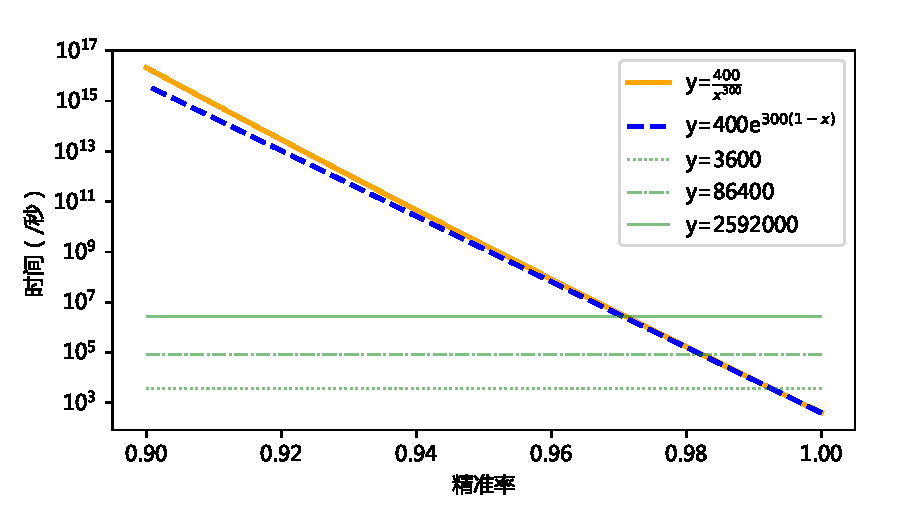
\includegraphics[width=\textwidth]{expotime}
%			\bicaption{\enspace 敏感信息估计值精确率对攻击时间期望的影响}{\enspace Impact of precision on the expectation of attack time}
%			\label{fig:expotime}
%		\end{center}
%	\end{figure}
%	
%	需要注意的是,求解算法$\mathcal S$要求\textbf{被利用的敏感信息估计值}的准确率是100\%,而没有要求\textbf{可利用的敏感信息估计值}准确率是100\%。又由于\corollaryref{cor:highbitinfo}和\corollaryref{cor:lowbitinfo},我们可以知道\textbf{可利用的敏感信息估计值}都是被预测为正例的\footnote{三段论。大前提,敏感信息都被预测为正例。小前提,可利用的敏感信息估计值是敏感信息。结论,可利用的敏感信息估计值都被预测为正例。}。既然所有\textbf{可利用的敏感信息估计值}都是被预测为正例的,那么\textbf{可利用的敏感信息估计值}的准确率就是精确率。又由于\textbf{可利用的敏感信息估计值}在\textbf{所有预测为正例的敏感信息估计值}中的分布是随机的,因此\textbf{可利用的敏感信息估计值}的准确率约等于\textbf{所有预测为正例的敏感信息估计值}的准确率,即\textbf{敏感信息估计值}精确率。
%	
%	因此,在敏感信息估计值精确率略小于100\%的情况下,可以多次尝试仅使用部分泄漏并使用$S$求解。如果选取到的部分泄漏恰好没有错误,那么求解算法能求解出实际私钥$\sk$。这样带来的代价是需要消耗更多时间才能恢复实际私钥。具体来讲,在敏感信息估计值精确率略小于100\%的情况下,使用多次尝试$S$的方法所消耗的时间会随着精确率的减小而成指数级增长,推导过程如\propositionref{prop:expotime}所示。\figureref{fig:expotime}展示了敏感信息估计值精确率略小于100\%的情况下多次尝试$S$的方法在理论上的技术效果,其中橙色实线表示恢复实际私钥的时间的期望,蓝色虚线表示使用指数函数可以对时间期望的下限做一个很好的估计,不同线型的绿色虚线表示攻击所能容忍的不同程度时间消耗(一小时、一天、一个月)。进一步分析可以知道,如果要求使用数学方法分别在一个月、一天、一小时内恢复实际私钥,那么通过侧信道攻击所恢复敏感信息估计值精确率分别需要达到97.12\%、98.22\%、99.27\%。
%
%	本研究的攻击点是ECDSA签名操作中数乘实现(\algorithmref{alg:improvesignscalar})中$\leakedmultiplier_i$的泄漏,侧信道攻击最终目标是恢复足够多可利用\footnote{足够多、可利用的具体标准取决于求解算法$\mathcal S$。对于本文使用的求解算法$S$,足够多指使用75条有可利用泄漏的签名构造方程,可利用指签名中的随机数泄漏连续4比特。}的签名中的一次性随机数$\nonce$的泄漏的情况下,提高敏感信息估计值精确率。侧信道攻击恢复敏感信息估计值精确率越高,求解实际私钥所需要调用$S$的次数就越少,攻击时间也就越少。侧信道攻击恢复随机数泄漏越多,求解出实际私钥的可能性就越大。

%	侧信道攻击智能卡ECDSA直到恢复实际私钥分为如下多个步骤。其中,步骤一可以通过改进采集环境或采集设备提升采集到的泄漏数量,步骤二通过改进侧信道攻击方法或降低置信度提升恢复的信息泄漏数量,步骤三需要通过更强的数学工具才可能在现有基础(见\apptableref{apptab:infoonsymbol})上进一步提升恢复敏感信息泄漏的比例,步骤四无法改进,步骤五可以通过使用更好的求解算法加以改进以减少攻击时间。
%	
%	\begin{enumerate}
%		\item [\textbf{步骤一}]采集多条签名以及对应的电磁迹;
%		\item [\textbf{步骤二}]从电磁迹中预测信息泄漏$\leakedmultiplier_i$的估计值$\hat \leakedmultiplier_i$;
%		\item [\textbf{步骤三}]从信息泄漏估计值$\hat \leakedmultiplier_i$计算某些敏感信息的估计值$\hat \nonce_i$;
%		\item [\textbf{步骤四}]从签名中过滤出所有有连续4比特泄漏的签名;
%		\item [\textbf{步骤五}]每次随机选择75条签名,利用签名以及其泄漏调用$S$求解直至求解成功。
%	\end{enumerate}
%	
%	对于步骤一,在现有实验条件下(见\tableref{tab:acquisitionpara})每条签名中数乘实现时长约50ms的电磁迹只能采集10ms,128次迭代只能采集到约30次(即$n_s\approx30$)。对于步骤二,使用通用数据增强方法提升恢复的信息泄漏数量。步骤三、四、五不在本研究范围内,提升效果的具体方法不予赘述。
%	
%	本研究不考虑进一步改进步骤一、三、四、五,这使得使用侧信道分析实现步骤二需要考虑如下难点:
%	
%	\begin{itemize}
%		\item 信息泄漏难以定位;
%		\item 敏感信息估计值精确率要求高\footnote{具体数值由电磁迹条数、电磁迹包含的迭代次数、从信息泄漏中恢复敏感信息泄漏的比例、求解算法$\mathcal S$对可利用敏感信息泄漏的定义、求解算法$\mathcal S$对敏感信息泄漏总量的需求、求解算法$\mathcal S$的运行时间、求解算法$\mathcal S$本身的成功率、可以容忍的攻击的时间消耗等多种因素共同决定。};
%	\end{itemize}

%	\subsection{量化指标选择}
%	
%	针对量化指标选择的问题,本研究使用了敏感信息泄漏估计真阳性率作为评价指标,计算方式如\equationref{eq:tpr}所示。本研究将敏感信息泄漏值$\nonce^{(i)}_j=0,i=0,1,\dots,T_a-1,j=0,1,\dots,n_s-1$的样本称为阳性样本,$\nonce^{(i)}_j=1,i=0,1,\dots,T_a,j=0,1,\dots,n_s-1$的样本称为阴性样本。据此可以定义真阳性、真阴性、假阳性、假阴性的样本。
%	
%	\begin{itemize}
%		\item [真阳性] 如果样本符合$\nonce^{(i)}_j=0,\hat \nonce^{(i)}_j=0$的条件,那么它是真阳性;
%		\item [真阴性] 如果样本符合$\nonce^{(i)}_j=1,\hat \nonce^{(i)}_j=1$的条件,那么它是真阴性;
%		\item [假阳性] 如果样本符合$\nonce^{(i)}_j=1,\hat \nonce^{(i)}_j=0$的条件,那么它是假阳性;
%		\item [假阴性] 如果样本符合$\nonce^{(i)}_j=0,\hat \nonce^{(i)}_j=1$的条件,那么它是假阴性。
%	\end{itemize}
%
%	\begin{equation}\label{eq:tpr}
%		TPR=\frac{TP}{TP+FP}
%	\end{equation}
%
%	在此基础上,本研究将真阳性、真阴性、假阳性、假阴性样本的样本个数分别记为TP、TN、FP、FN,它们的关系如\tableref{tab:cmatrixk}所示。敏感信息泄漏估计真阳性率的计算方式如\equationref{eq:tpr}所示,它适用于不能容忍将阴性样本错误估计为阳性的情况。就本研究而言,因为ECDSA本身的特性以及后续格方法的特殊要求,假阴性的数量或比例在不超过阈值的情况下不会对求解私钥的效率和正确性产生影响,证明见\propositionref{prop:highalpha}。因此,虽然真阳性率作为评价指标的场景少见,但它适合作为本研究评价指标。
%
%	\begin{table}[!h]
%		\bicaption{\enspace $\nonce_j$的混淆矩阵}{\enspace Confusion matrix of $\nonce_j$}
%		\label{tab:cmatrixk}
%		\centering
%		%\footnotesize% fontsize
%		%\setlength{\tabcolsep}{4pt}% column separation
%		%\renewcommand{\arraystretch}{1.2}%row space
%		\begin{tabular}{c|c|cc}
%			\hline
%			\multicolumn{2}{c|}{\multirow{2}{*}{样本数}} & \multicolumn{2}{c}{$\hat \nonce^{(i)}_j$(估计值)} \\
%			\cline{3-4}
%			\multicolumn{2}{c|}{}& 0& 1 \\
%			\hline
%			\multirow{2}{*}{$\nonce^{(i)}_j$(值)} & 0 & TP & FP \\
%			%\cline{2-5}
%			& 1 & FN & TN \\
%			\hline
%		\end{tabular}   
%	\end{table}
}
	
	%\subsection{分析技术选择}
	\subsection{\yuchuli}\label{subs:selectpoi}

	直接使用深度学习模型对电磁迹进行DL-SCA在理论上可行,但是在实践中所需的计算量巨大,本文实验环境需要使用315天才能完成深度学习模型的训练。为了解决这个问题,本研究选择提取POIs,使得在尽可能保留敏感信息泄漏的同时减少信息泄漏的维数,对应的深度学习模型所需的存储空间和训练的计算量可以有效地减小,使用现有的计算资源足够进行DL-SCA。这样做还带来一个额外的好处:电磁迹可以根据POIs对齐结果,模数转换评价对齐程度可以直观地反映特征点提取是否准确。
{	
%	本研究提出了一种基于时间模板的两阶段对齐解决信息泄漏难以定位的问题;本文应用了前一章的通用数据增强方法提升敏感信息估计值精确率。
	
%	侧信道分析的第一个难点在于,敏感信息是$\tilde{k}_i$没有直接泄漏,这使得从理论上讲不可能从电磁迹泄漏中恢复所有敏感信息。从一条签恢复的恢复的敏感信息越少,就需要使用越多签名构造方程才可能求解出私钥。
%	
%	
%	即使以100\%的成功率恢复所有泄漏的$t_i$,也会因无法分辨泄漏来自于算法的哪个分支(\algorithmref{alg:improvesignscalar}第5、8行),从而在理论上不能完全恢复$\tilde k_i$的信息,进而不能恢复随机数$k$的所有泄漏\footnote{因为$\left\{\tilde{k}_0,\tilde{k}_1,\dots,\tilde{k}_i,\dots, \tilde{k}_{l-1}\right\}$是$k$的编码形式,所以恢复某些$\tilde k_i$的比特等价于恢复随机数$k$的等量比特。因为$(k_0k_1k_3\dots k_{257})_2$是$k$的二进制表示,所以恢复某些$k_i$也等价于恢复随机数$k$的等量比特。}。\tableref{tab:infoonsymbol}总结了从$t_i$中所恢复的$\tilde k_i$和$k$的信息。从\tableref{tab:infoonsymbol}中可以归纳出这样的结论:
%	
%	\begin{itemize}
%		\item 如果攻击者知道$t_i=1$(有$\frac38$的概率发生),那么攻击者可以推断$\tilde k_i$的高比特是0,即$k_i=0$(见\algorithmref{alg:encodek}),无法推断$\tilde k_i$的低比特。
%		\item 如果攻击者知道$t_i=2$(有$\frac5{16}$的概率发生),那么攻击者可以推断$\tilde k_i$的低比特是0,即$k_{i+129}=0$,无法推断$\tilde k_i$的高比特。
%		\item 如果攻击者知道$t_i=3$(有$\frac5{16}$的概率发生),那么攻击者无法推断$\tilde k_i$的任意比特。
%	\end{itemize}
%	
%	
%	侧信道攻击所能恢复的是$t_i$的数值,构造方程的签名中的随机数泄漏是$\tilde k_i$的数值,这两个不能完全对应。依据前两条结论从$t_i$中推断出的随机数$k$的某些比特的值就是攻击者可以完全确定的所有随机数$k$的泄漏。这些泄漏随机地分布在随机数$k$所有位置。因此攻击者
%		
%	从\tableref{tab:infoonsymbol}中归纳的信息可以看出,对于任意一条签名中随机数$k$的任意一个比特$k_i$,不可能使用侧信道攻击得出这样的结论:有超过100\%的把握认为$k_i=1$。
%	
%	实际上,在采集的电磁迹受限的情况下,侧信道攻击恢复随机数泄漏多和侧信道攻击恢复随机数泄漏的准确率高两个目标是互相冲突的。原因在于,在采集的电磁迹受限下,可以很容易地通过提高置信度实现提高侧信道攻击恢复随机数泄漏的准确,但是这样一来会减少侧信道攻击恢复随机数泄漏。
	
	
%	\section{智能卡ECDSA算法实现信息泄漏预处理方法研究}
%	%$\forall 0\le i<T,\forall 0\le j<n_s\leakedmultiplier^{(i)}_j$估计值$\hat\leakedmultiplier^{(i)}_j$的泄漏是信息泄漏。$\forall 0\le i<T,\forall 0\le j<n_s,\tilde \nonce^{(i)}_j,\nonce^{(i)}_j,\nonce^{(i)}_{j+129},\mathbb 1_{\leakedmultiplier^{(i)}_j=1}$数值的泄漏是信息泄漏,其中$\mathbb 1$是示性函数,取值范围为0或1,它取1当且仅当下标表示的事件发生。可利用的敏感信息指的是$\tilde \nonce_i,0<i<258$数值的泄漏
%	
%	%//TODO:
%	侧信道攻击需要预测敏感信息的准确率高,但是对于以准确率作为评价恢复信息泄漏$\leakedmultiplier_i$效果的指标不合理。从\apptableref{apptab:infoonsymbol}可以看出攻击者只能从$\hat\leakedmultiplier_i$的取值中对一次性随机数$\nonce$的某个比特$\nonce_i$做出$\hat\nonce_i=0$的估计,而无法对任意比特做出$\hat\nonce_i=1$的估计。因此评价恢复$\leakedmultiplier_i$信息泄漏效果时,只用考虑在预测$\hat\leakedmultiplier_i=1$的条件下尽可能达成$\leakedmultiplier_i=1$、预测$\hat\leakedmultiplier_i=2$的条件下尽可能达成$\leakedmultiplier_i=2$,而不用考虑在预测$\hat\leakedmultiplier_i=3$的条件下尽可能达成$\leakedmultiplier_i=3$。为了方便,我们用\tableref{tab:cmatrixt}所列举的表项说明这种变化,评价指标由$accuracy=\frac{\mathrm{TP}1+\mathrm{TP}2+\mathrm{TP}3}{\mathrm{TP}1+\mathrm{FP}1_2+\mathrm{FP}1_3+\mathrm{FP}2_1+\mathrm{TP}2+\mathrm{FP}2_3+\mathrm{FP}3_1+\mathrm{FP}3_2+\mathrm{TP}3}$变为$\frac{\mathrm{TP}1+\mathrm{TP}2}{\mathrm{TP}1+\mathrm{FP}1_2+\mathrm{FP}2_1+\mathrm{TP}2+\mathrm{FP}3_1+\mathrm{FP}3_2}$。又由于本研究使用的求解算法$S$不考虑低位的泄漏,因此本研究只考虑在预测$\hat\leakedmultiplier_i=1$的条件下尽可能达成$\leakedmultiplier_i=1$。我们还是用\tableref{tab:cmatrixt}所列举的表项说明这种变化,评价指标由$\frac{\mathrm{TP}1+\mathrm{TP}2}{\mathrm{TP}1+\mathrm{FP}1_2+\mathrm{FP}2_1+\mathrm{TP}2+\mathrm{FP}3_1+\mathrm{FP}3_2}$进一步变为$\frac{\mathrm{TP}1}{\mathrm{TP}1+\mathrm{FP}2_1+\mathrm{FP}3_1}$。根据\corollaryref{cor:highbitinfo}可以知道,\tableref{tab:cmatrixt}所列举的表项表述的公式$\frac{\mathrm{TP}1}{\mathrm{TP}1+\mathrm{FP}2_1+\mathrm{FP}3_1}$实际上就是\tableref{tab:cmatrixk}所列举的表项表述的\equationref{eq:precision}。因此我们将$\frac{\mathrm{TP}1}{\mathrm{TP}1+\mathrm{FP}2_1+\mathrm{FP}3_1}$称为信息泄漏估计值$\hat\leakedmultiplier_i$的精确率,它和敏感信息估计值$\hat\nonce_i$的精确率在数值上是恒等的。
%	
%	信息泄漏指的是$\leakedmultiplier_i$的泄漏。
}
	
	通常来说,提取POIs是通过对电磁迹进行对齐,再从对齐结果中选取POIs。但就本研究而言,一条签名的电磁迹采样点个数达到$5\cdot10^{7}$,但一条电磁迹中包含150组、共7500个特征不明显的POIs,且不同组的50个POIs不连续。现有的对齐方法无法同时满足高效和准确的需求,因此也不能高效和准确的完成POIs的提取。电磁迹中每处信息泄漏的POIs少(约50个采样点),使用基于与单处信息泄漏相关系数的静态对齐会因为产生大量误报\footnote{原本不是敏感信息泄漏,但是静态对齐结果显示是敏感信息泄漏。}而无法准确提取POIs。电磁迹中每处信息泄漏之间引入了随机延迟,使用基于与多处信息泄漏相关系数的静态对齐会使得出现大量漏报\footnote{原本是敏感信息泄漏,但是静态对齐结果显示不是敏感信息泄漏。}而过滤掉信息泄漏。电磁迹中每处信息泄漏间隔的时间长,使用动态对齐会因为计算量巨大而不能高效提取POIs。
	
	本研究提出\yuchuli 技术。它的核心思想是筛选电磁迹和卷积核卷积的极值点\footnote{极大值点或极小值点。在一个有定义的点的周围的点也都有定义,且在这个点的左右邻域的函数值都小于这个点的值,则该点为极大值点,同理为极小值点。},将最匹配时间模板的极值点组合记为POIs。
%	本研究提出一种基于时间模板的\yuchuli 预处理技术可以高效准确地从目标电磁迹中提取POIs。它大致分为如下两个阶段:
%	
%	\begin{itemize}
%		\item [\textbf{阶段一,高效确定信息泄漏范围}]分块计算方差,对分块结果依次进行模数转换、去抖动、一维高斯模糊、模数转换、去抖动,定位到泄漏的大致范围,将电磁迹初步划分为电磁子迹;
%		\item [\textbf{阶段二,准确确定信息泄漏位置}]在电磁子迹中计算不同偏移程度下与一处信息泄漏的模板的协方差,筛选出一定数量的极值点,枚举可能极值点的组合检查是否匹配信息泄漏的时间模板。
%	\end{itemize}
	在执行\yuchuli 之前,需要使用分块方差以及模数转换、去抖动、一维高斯模糊的信号处理技术缩小POIs范围,提高\yuchuli 效率。\yuchuli 之前的这个预计算操作称为\poifanwei 技术。
	
	
	%可以认为智能卡ECDSA算法实现信息泄漏预处理的时间消耗和采样点个数线性相关。在阶段一,本研究在保留信息泄漏特征的情况下使用时间复杂度低($\Theta(M)$)的算法高效确定信息泄漏范围;在阶段二,本研究使用时间复杂度高($\Theta(n_sM_s\log M_s)$)的算法准确确定信息泄漏位置。算法复杂度中的$M,n_s,M_s$分别表示电磁迹采样点个数、电磁迹包含的迭代次数、一次迭代所对应的电磁子迹\footnote{本文将一次迭代所对应的POI附近的电磁迹称为电磁子迹(Subtrace)的采样点个数,这么命名的原因是它实际上就是电磁迹的一部分。}的采样点个数。虽然阶段二的算法复杂度较高,但是算法复杂度中的变量的数值更小(对于本研究,$M=5\cdot10^7,n_s=30,M_s=18000$),所以在当前数据范围内阶段二时间消耗也是很小的。因此,预处理时间消耗中执行阶段一的时间消耗占主导作用,预处理时间消耗和电磁迹采样点个数线性相关。

	\textbf{采用\poifanwei 技术确定特征点范围。}	
	\poifanwei 技术使用降采样的思想,以线性时间复杂度定位到POIs的大致范围,范围从50000000采样点减小到18000采样点。一条50000000个采样点的电磁迹含有30组POIs,每组POIs互不连续(坐标之差超过1000000采样点),一组POIs包括五个不连续的POIs(每个POI与同组的其他POI的距离在2300至3500采样点之间)。\poifanwei 技术首先依据信息泄漏部分电磁场强度变化大的特性分块计算方差可以降采样并使得信息泄漏处依然保留的特征。接着依次使用模数转换、去抖动、模糊、模数转换、去抖动的方法组合电磁迹更多信息得到的用于确定特征点范围的辅助信息。这个辅助信息是一个01数列,我们将其视为方波的采样结果。此时电磁迹可以依据计算出的辅助信息较为准确地划分每次迭代\footnote{具体划分方法取决于模数转换、去抖动、一维高斯模糊、模数转换、去抖动的参数。对于本研究的电磁迹和函数参数,每过8个方波,数乘实现会在上升沿进入下一次迭代。},且每次迭代中有多个锚点辅助定位泄漏的大致范围\footnote{锚点即为方波的上升沿或下降沿时刻。对于本研究的电磁迹和函数参数,每次迭代中第一个方波的下降沿到泄漏的位置相隔的采样点个数一定在区间$[8.0\cdot10^{4},9.8\cdot10^{4}]$以内。}。
	
	分块方差的实现见\algorithmref{alg:calcvar},它依据参数$w_d$对电磁迹分块并计算每块中所有电磁场强度样本值的方差,在信息泄漏处依然保留的特征的情况下进行降采样以降低后续操作的时间复杂度,其本身时间复杂度$\Theta(M)$。分块计算方差的输出结果可以视为一个降采样后的波。
	
	模数转换的实现见\algorithmref{alg:quantize},它依据阈值参数$th$将非01数列(模拟信号)转换为01数列(数字信号)以便于后续操作和分析,其时间复杂度为$\Theta(N_X)$。
	
	本研究从硬件设计中对物理按键去抖动的硬件代码得到启发而设计了去抖动函数。函数通过缓存一段长度的数列实现排除偶然噪声(采样点个数少于$w_a$的方波)的干扰但保留主体波形,它的实现见\algorithmref{alg:antijitter}。它通过检查当前位置数据以及之前的$w_a-1$个数据,综合判断应该如何解析当前状态并记录。去抖动会对数据引入延迟,去抖动后方波的上升沿和下降沿会相比于去抖动前延后$w_a$个采样点,有时需要进行校正。去抖动时间复杂度为$\Theta(N_X)$。
	
	本研究从图像处理中的模糊操作得到启发而设计了模糊函数。函数计算窗口大小为$2w_g+1$的二项分布的卷积核,扫描数列中的每个样本,用卷积核确定的邻域内的样本的加权平均数替代当前样本的值,它的实现见\algorithmref{alg:gaussblur}。它作为上一步去抖动函数的补充,进一步排除噪声的干扰并保留主体波形。模糊函数本质上是实现了卷积,为了使得模糊后的数列与输入的数列大小相同,卷积使用了same\footnote{使用文档见\href{https://numpy.org/doc/stable/reference/generated/numpy.convolve.html}{numpy.convolve}。}模式。模糊函数的时间复杂度为$\Theta(w_gN_X)$。
	
	执行模糊操作之后,需要再次执行模数转换和去抖动,利用这之后的结果才能确定特征点范围。

	\poifanwei 最耗费时间的是模糊操作。如果不进行分块那么$N_X=M$,它的时间复杂度$\Theta(w_gN_X)=\Theta(w_gM)$是难以接受的。分块计算方差后,每条电磁迹长度为$M$的采样点被压缩成了长度为$N_X=\left\lfloor\frac{M}{w_d}\right\rfloor$的数列,模糊的时间复杂度下降为$\Theta(w_gN_X)=\Theta(\frac{w_g}{w_d}M)$。只要$w_g<w_d$,\poifanwei 的时间复杂度就可以由$\Theta\left( w_gM\right) $变为$\Theta(M)+\Theta\left( \frac{M}{w_d}\right) +\Theta\left( \frac{M}{w_d}\right) +\Theta\left( \frac{w_g}{w_d}M\right) +\Theta\left( \frac{M}{w_d}\right) +\Theta\left( \frac{M}{w_d}\right) =\Theta(M)$。对于本研究,$M=5\cdot10^7,w_d=360,w_g=300$。
	
	通过应用\poifanwei 技术,可以完全确定电磁迹30组POIs中,每组POIs都在长度为18000个采样点的区间内。%此时对$n_s$次迭代中包含信息泄漏的电磁迹进行subsub基于与单处信息泄漏相关系数的静态对齐,还是不能保证5处包含信息泄漏的电磁迹会恰好对应相关系数的前五个极值点。
	
	%本研究在前一个阶段最后步骤上改动了两个实现细节以实现阶段二,一个是计算相关系数改为计算协方差,另一个是将取前5个相关系数极值点改为取前$m$个相关系数极值点,枚举其中的5个并逐一使用实现构造的时间模板进行检查。
	
	%计算协方差而不是相关系数的原因是,信息泄漏对应的电磁场变化幅度较大,但是计算相关系数会丢弃这种特征。使用协方差就是在使用相关系数的基础上一并考虑了信息泄漏电磁迹本身的方差,因此使得信息泄漏更容易被区分。除此之外,将相关系数改为计算协方差后,只要模板的所有点的均值为0,计算所有采样点邻域的相关系数就可以直接用卷积实现,这可以减少程序的时间消耗。计算协方差的算法复杂度是$\Theta(w_tN_X)$,其中$w_t$是模板宽度,$N_X$是信息泄漏所在区间的宽度,对于本研究$w_t=30,N_X=18000$。
	\textbf{采用\yuchuli 技术确定特征点坐标。}
	\yuchuli 技术使用静态对齐和模板匹配的思想,准确提取特征点坐标,可以达到与人工标注相当的效果,偏差不超过10个采样点。\yuchuli 技术首先构造模板(为了与后文的时间模板加以区分,将其称为电磁模板)和时间模板,计算每个特征点范围内的电磁信号和电磁模板的卷积(逐点的相关系数),取卷积的前$m$个邻域互不相交的极值点,枚举所有$m$选五的组合,逐一检验每个极值点组合与时间模板的匹配程度,选择最匹配的组合所对应的极值点作为特征点。其中,参数$m$可以依据具体情况选择,$m$越大那么执行时间越长,结果也越准确。
	
	取前$m$个极值点的实现如\algorithmref{alg:maxpoint}所示,其中函数的输入$\Vector X$应当是计算出的协方差数列,极值点定义中的"邻域"通过阈值$th$加以描述。对于本研究,$th=100,m=9$。算法首先对数列的绝对值进行排序,依次检查第$i$大的绝对值,如果它不在当前所有极值点的邻域内,那么它就是一个新的极值点,把它加入集合$\mathcal M$。最后,假如极值点个数达到需求,程序结束并返回极值点的集合。函数的算法复杂度是$\Theta(N_X\log N_X)$,其中$N_X$是信息泄漏所在区间的宽度,对于本研究$N_X=18000$。
	
	枚举$m$个极值点中所有的5个极值点两两配对的组合并计算坐标之差,逐一使用实现构造的时间模板进行匹配的实现如\algorithmref{alg:checkdelta}所示,其中函数的输入$\mathcal M$应当是上一个算法输出的采样点集合,$\mu_{5\times5},\sigma_{5\times5}$是预计算的模板,它们刻画了POIs横坐标之间的时间的规律,如果极值点之间的距离可以匹配模板,那么我们认为选出的极值点恰好就对应POIs。实际验证时发现存在无论如何枚举$m$个极值点中的5个都不能匹配模板的问题(算法返回空集),因为这种情况发生的概率很小,我们直接丢弃当前迭代所对应的电磁迹,认为这一次迭代不存在泄漏(也可以直接将这一次迭代对应的敏感信息泄漏估计为阴性样本)。函数的算法复杂度是$\Theta\left( \begin{pmatrix}m\\5\end{pmatrix}\begin{pmatrix}5\\2\end{pmatrix}\right) =\Theta(m^5)$。
	
	\begin{breakablealgorithm}
		\caption{时间模板匹配}\label{alg:checkdelta}
		\begin{algorithmic}[1]
			\Statex \textbf{输入:} $\mathcal M$:$m$个采样点位置的集合
			\Statex \textbf{输入:} $\mu_{5\times5}$:预计算的模板,极值点的差的均值
			\Statex \textbf{输入:} $\sigma_{5\times5}$:预计算的模板,极值点的差的标准差
			\Statex \textbf{输出:} $\mathcal A$:最先匹配的极值点组合
			\For{$\mathcal A\subset M$}
			\If {$\left\vert\mathcal A\right\vert=5$}
			\State $\{a_0,a_1,a_2,a_3,a_4\}=\mathcal A,a_0<a_1<a_2<a_3<a_4$
			\If{$\forall 0\le i<j<5,\vert a_j-a_i-\mu_{i,j}\vert<3\sigma_{i,j}$}
			\State \Return $\mathcal A$
			\EndIf
			\EndIf
			\EndFor
			\State \Return $\phi$
		\end{algorithmic}
	\end{breakablealgorithm}
	%\subsection{智能卡ECDSA算法实现信息泄漏预处理方法的实证研究}
	
	%\textbf{电磁迹预处理。}
	%在初步验证所提方法有效性的基础上,将新提出的方法应用于双界面商用智能卡ECDSA算法实现分析场景中,对采集的电磁迹进行预处理。这样一来,在尽可能保留敏感信息泄漏的同时减少信息泄漏的维数,对应的深度学习模型可以有效地缩小,使用以现有的计算资源进行DL-SCA变得可行。
	
	%\section{通用数据增强方法在ECDSA算法实现分析中的应用}
	%\subsection{ECDSA实现数据集}
	\textbf{构造数据集。}本研究在\tableref{tab:acquisitionpara}所示的采集条件下采集了数据集。之后需要应用\yuchuli 技术构造数据集,用于后续的建模和分析。%但是由于针对ECDSA的侧信道分析与针对AES等分组密码算法的侧信道分析方法有较大差异,直接进行DL-SCA的计算开销过大,因此需要对数据集进行处理才能将更好地适配深度学习模型。
	
%	除此之外,在$T_a$条电磁迹共约$T_an_s$次迭代所对应的电磁子迹中,实际上只有比例约为$\frac34$的电磁子迹(因为执行了\algorithmref{alg:improvesignscalar}的第5、6行而)会包含对应的敏感信息泄漏,剩下的比例约为$\frac14$的电磁子迹(因为执行了\algorithmref{alg:improvesignscalar}的第8、9行而)不包含对应的敏感信息泄漏。
%	
%	攻击者无法区分这两种电磁子迹。如果攻击者将不含敏感信息泄漏的电磁子迹误判为包含敏感信息泄漏,运用格方法成功恢复私钥的概率会随着这种误判次数的增加程指数级减小。因此攻击者需要找到一个不完全依赖于“电磁迹一定要包含敏感信息泄漏”的方法,使得无论电磁子迹是否包含敏感信息泄漏,攻击者所恢复的敏感信息泄漏都应该尽可能准确。分析\algorithmref{alg:improvesignscalar}可以知道,无论函数在循环体中执行哪个分支,\corollaryref{cor:highbitinfo}和\corollaryref{cor:lowbitinfo}始终成立。因此,攻击者可以由\corollaryref{cor:highbitinfo}和\corollaryref{cor:lowbitinfo}预先总结出依据泄漏$\leakedmultiplier_j$(见\algorithmref{alg:improvesignscalar})计算敏感信息泄漏估计值$\hat \nonce_j$的表格,如\apptableref{apptab:infoonsymbol}所示,每次依据侧信道分析结果查表即可。
%	
%	\begin{corollary}\label{cor:highbitinfo}
%		如果$\leakedmultiplier_j=1$,那么$\nonce_j=0$。
%	\end{corollary}
%	\begin{proof}
%		证明逆否命题即可。如果$\nonce_j\neq0$,那么$\nonce_j=1$,$\tilde \nonce_j=2$或$\tilde \nonce_j=3$。当$\tilde \nonce_j=2,\leakedmultiplier_j=2\neq1$。当$\tilde \nonce_j=3,\leakedmultiplier_j=3\neq1$。因此,如果$\nonce_j\neq0$,$\leakedmultiplier_j\neq1$。
%	\end{proof}
%
%	\begin{corollary}\label{cor:lowbitinfo}
%		如果$\leakedmultiplier_j=2$,那么$\nonce_{j+129}=0$。
%	\end{corollary}
%	\begin{proof}
%		证明逆否命题即可。如果$\nonce_{j+129}\neq0$,那么$\nonce_{j+129}=1$,$\tilde \nonce_j=1$或$\tilde \nonce_j=3$。当$\tilde \nonce_j=1,\leakedmultiplier_j=1\neq2$。当$\tilde \nonce_j=3,\leakedmultiplier_j=3\neq2$。因此,如果$\nonce_{j+129}\neq0$,$\leakedmultiplier_j\neq2$。
%	\end{proof}
	
			
	%即使是评估者也只能知道比例约为$\frac34$的信息泄漏$\leakedmultiplier_i$真实值,对于剩下的电磁子迹,攻击者不知道信息泄漏真实值,因此也无法判断它们哪些是正例,那些是反例。为了排除潜在的系统误差,我们也需要对数据集进行处理。
	
	对于评估者而言,他知道敏感信息而可以区分这两种电磁子迹,因此在量化评价分析技术的时候可以选择“最有利于攻击者的情况”进行评估。如果在这种情况下攻击者都难以完成攻击,那么说明ECDSA实现具有一定抵抗侧信道分析的能力。\algorithmref{alg:filter}给出了评估者构造最有利于攻击者的数据集的流程,它从电磁迹中提取包含信息泄漏的电磁子迹,并处理好了相应的标签以用于深度学习。使用这种方法能提取POIs还避免构造出的数据集有不对齐的问题,一条电磁迹的采样点数也由$5\cdot10^7$减小到300,这使得DL-SCA变得可行。在5000条电磁迹中,提取出了$cnt\approx100000$次迭代所对应的电磁子迹作为数据集,即$L_0^{out}$中有$cnt$条电磁子迹、$L_1^{out}$中有$cnt$条电磁子迹……这意味着ECDSA实现有多处操作与敏感信息泄漏$\tilde \nonce_j$有关\footnote{具体关系因为缺少相关资料而无法证实也无法证伪。本研究的猜测是,硬件从外存中取出数据到寄存器时,因为数据过大(数据为两个256比特的数,但通用寄存器位宽相对较小,比如64比特),需要执行多个周期,因此地址线的数据会在多个时刻都有泄漏。}。
	
	\begin{breakablealgorithm}
		\caption{有效电磁子迹提取}\label{alg:filter}
		\begin{algorithmic}[1]
			\Statex \textbf{输入:} $L$:$T_a$条各包含$n_s$次迭代的信息泄漏的电磁迹
			\Statex \textbf{输入:} $\sk$:ECDSA私钥
			\Statex \textbf{输入:} $q$:椭圆曲线的阶
			\Statex \textbf{输入:} $P$:$T_a$组ECDSA签名消息的哈希值和签名
			\Statex \textbf{输出:} $L^{out}$:过滤出的电磁子迹
			\Statex \textbf{输出:} $Label^{out}$:过滤出的电磁子迹对应的敏感中间值
			\Statex \textbf{输出:} $cnt$:过滤出的电磁子迹条数
			\State $L^{out}:=\left[ [],[],[],[],[]\right] $\Comment{五组电磁子迹,对应于五处泄漏位置}
			\State $Label^{out}:=[]$
			\State $counter:=0$
			\For {$i:=0,\dots,T_a-1$}
				\State $r:=p^{(i)}.r$\Comment{第$i$组ECDSA签名}
				\State $s:=p^{(i)}.s$\Comment{第$i$组ECDSA签名}
				\State $hsh:=p^{(i)}.hsh$\Comment{第$i$组ECDSA签名消息的哈希值}
				\State $\nonce:=s^{-1}(hsh+r\sk)\bmod q$
				\State 计算$\nonce$长度为129的编码形式$\left\{\tilde{\nonce}_0,\tilde{\nonce}_1,\dots,\tilde{\nonce}_j,\dots, \tilde{\nonce}_{128}\right\}$
				\For{$j:=1,\dots,n_s$}
					\If {$\tilde{\nonce}_j>0$}
						\State 确定第$(j-1)$次迭代对应的信息泄漏范围
						\State 确定第$(j-1)$次迭代对应的POIs横坐标$\mathcal A$
						\If {$\mathcal A\neq\phi$}
							\State $\{a_0,a_1,a_2,a_3,a_4\}=\mathcal A,a_0<a_1<a_2<a_3<a_4$
							\State 从位置$a_0$提取电磁迹,加入到$L_0^{out}$中
							\State 从位置$a_1$提取电磁迹,加入到$L_1^{out}$中
							\State 从位置$a_2$提取电磁迹,加入到$L_2^{out}$中
							\State 从位置$a_3$提取电磁迹,加入到$L_3^{out}$中
							\State 从位置$a_4$提取电磁迹,加入到$L_4^{out}$中
							\State 将$\left\lfloor\tilde{\nonce}_j/2\right\rfloor$加入到$Label^{out}$中\Comment{只利用$\tilde{\nonce}_j$的高比特}
							\State $cnt:=cnt+1$
						\Else
							\State continue
						\EndIf
					\Else
						\State continue
					\EndIf
				\EndFor
			\EndFor
		\end{algorithmic}
	\end{breakablealgorithm}
	
	\subsection{\shujuzengqiang}\label{subs:useagmt}
	DL-SCA通常假设攻击者能够从目标设备上采集到充足的样本,以进行模型训练和实施攻击。但就本研究而言,为了满足前提条件,需要耗费大量时间进行电磁迹的采集和预处理。采集5000条目标双界面商用智能卡ECDSA电磁迹就需要1天,从电磁迹中提取POIs并构造数据集还需要3天时间。本研究的实验环境下,DL-SCA的训练时间只有不到10分钟,远少于采集电磁迹和预处理的时间。
	
	如果在取得的效果相当的情况下,以增加DL-SCA的训练时间作为代价,大幅度减小采集电磁迹和预处理的时间,也是能减少完成侧信道分析的总时间的。
	
	本研究使用\chapref{chap:search1}提出的面向基于深度学习侧信道分析的数据增强方法,以增加少量数据增强时间作为代价,提高DL-SCA真阳性率。
	%\subsection{实验设置}
	\textbf{主控制器设置。}
	这部分设置与\subssref{subss:controllersettings}几乎相同。在使用猜测熵收敛速度作为攻击代价时,模拟退火的目标是最小化\equationref{eq:mycost}中的$convrate$。但是在使用信息泄漏估计值精确率(见本小节\textbf{攻击评估单元设置})作为攻击代价时,模拟退火的目标是最大化\equationref{eq:precision}中的$precision$。两个优化目标相反,因此需要对代码做细微调整。具体来说,\algorithmref{alg:saincontroller}的第9、14、19行的条件判断表达式应当分别由$cost-newcost\ge0$、$p<e^{\frac{cost-newcost}{temp}}$、$mincost\ge cost$调整为$cost-newcost\le0$、$p<e^{\frac{newcost-cost}{temp}}$、$mincost\le cost$。
	
	\textbf{数据增强单元设置。}
	这部分设置与\subssref{subss:cdasettings}一致。
	
	\textbf{深度学习模型设置。}
	深度学习模型选择了与\tableref{tab:cnnhyperpara}中攻击ASCADf(N=50)数据集的网络几乎相同的网络超参数,来说明基于通用数据增强方法的框架有效是因为多个组件共同作用而不是某一个组件使得DL-SCA性能大大提升。
	网络超参数基本相同,但训练轮次从50减到了20,这是通过深度学习验证阶段发现的针对ECDSA电磁子迹的一个优化点。输入样本的大小从700调整为300,这是因为AECADf(N=0)数据集对应的一条能量迹采样点个数为700,本研究使用的一条电磁子迹采样点个数为300。
	
	%深度神经网络的输入层大小调整为300,使用5000个电磁子迹进行20轮次的训练时计算量达到$1.6\cdot10^{13}$浮点运算次数(Floating Point Operations,FLOP),使用现有实验环境需要消耗8分钟。假如不进行\yuchuli 预处理操作,输入层大小需要设置为50000000,使用167条电磁迹(对应于5000条电磁子迹)进行20轮次的训练时计算量达到$8.7\cdot10^{16}$FLOPs,使用现有实验环境理论上需要消耗315天。
	
	\textbf{攻击评估单元设置。}
	在本研究中了,使用精确率作为攻击代价,计算公式如\equationref{eq:precision}所示。	
	
	\begin{equation}\label{eq:precision}
		precision=\frac{\vert\{i:0\le i<T_a,\theta^{(i)}>0.5,Label^{(i)}=0\}\vert}{\vert\{i:0\le i<T_a,\theta^{(i)}>0.5\}\vert}
	\end{equation}
	
	\noindent 其中$\hat\theta^{(i)}$表示深度学习模型所预测的第$i$个样本对应的标签为0的概率\footnote{因为是二分类,对应的标签为1的概率为$(1-\hat\theta^{(i)})$,即深度学习模型所预测的第$i$个样本的标签概率向量为$\begin{bmatrix}\hat\theta^{(i)}&1-\hat\theta^{(i)}\end{bmatrix}$。},$Label^{(i)}$表示第$i$个样本的真实标签(要么等于0,要么等于1)。精确率计算了预测标签为0的概率大于0.5的样本中,真实标签为0的样本所占的比例。
	
	精确率是深度学习中比较常见的评价指标,它是真阳性率的一种特殊情况。如果估计是使用的极大似然估计(且类别数为2),那么真阳性率与精确率完全一致;如果估计使用的其他估计方法,那么真阳性率与精确率不一致。
	
	因此,采用数据增强后,DL-SCA的训练阶段调整为\figureref{fig:mydlscatestecdsa}的形式。
	
	\begin{figure}[!h]
		\centering
		\begin{tikzpicture}[node distance=45pt, auto]
		% 定义节点样式
		\tikzstyle{reg} = [rectangle, draw,text centered]
		\tikzstyle{block} = [draw, rounded corners,align=center]
		\tikzstyle{data} = [draw, trapezium, trapezium left angle=70, trapezium right angle=110,align=center]
		\tikzstyle{arrow} = [thick,->,>=stealth]
		
		% 绘制节点
		\node [reg] (hyperparareg) {超参数寄存器};
		\node [block,below of =hyperparareg] (trained) {深度神经网络};
		\node [reg, left=70pt of trained] (parareg) {参数寄存器};
		\node [data, below of=trained] (dataset) {数据集};
		\node [block, right=50pt of dataset] (valacc) {机器学习\\指标计算器};
		
		%\node [block, below of=valacc, xshift=2cm] (testacc) {测试集准确率计算器};
		
		% 绘制箭头
		\draw [arrow] (dataset) -- node[right] {测试数据} (trained);
		\draw [arrow] (dataset) -- node[pos=0.5,below] {测试标签} (valacc);
		%\draw [arrow] (dataset) -- node[above] {测试数据} (pretrained);
		\draw [arrow] (trained) -| node[above] {测试数据的预测结果} (valacc);
		\draw [arrow] (hyperparareg) -- node[right]{网络超参数}(trained);
		\draw [arrow] (parareg) -- node[above]{神经元参数}(trained);
		\draw [arrow] (valacc) --node[midway, above] {精确率$precision$} ++(0:110pt);
		\end{tikzpicture}
		\bicaption{\enspace 攻击ECDSA的深度学习验证阶段}{\enspace DL test phase for SCA on ECDSA}
		\label{fig:mydlscatestecdsa}
	\end{figure}
	\subsection{\jiashejianyanguji}
	模板类攻击通常为了最小化错误判定的概率而使用极大似然判定准则估计敏感信息泄漏或密钥。但目标双界面商用智能卡上ECDSA实现本身较为特殊,这导致侧信道分析在一定的限度内只需要减少敏感信息泄漏取伪错误(出现假阳性),而弃真错误(出现假阴性)不会对恢复私钥的效率和正确性产生影响。
	
	本研究提出了\jiashejianyanguji 方案,最小化取伪错误发生的概率。具体来说,对于每一个敏感信息泄漏估计,假设$\nonce^{(i)}_j=0$并计算统计量$\theta$进行检验。统计量$\theta$的计算方法就是使用深度学习模型预测敏感信息泄漏概率向量,显著性水平$\alpha$依据由电磁迹条数、一条电磁迹包含的迭代次数、最终运用的格方法共同决定,统计量阈值$\theta_{\alpha}$由显著性水平决定。
	
	%利用深度学习模型输出得敏感信息泄漏概率向量对敏感信息泄漏进行估计时,无论采用何种估计方法,理论上会存在两种错误的可能性:弃真错误和取伪错误。对于以对称加密算法(如AES)实现为攻击目标侧信道分析而言,需要同时减少弃真错误和取伪错误以提高所恢复的敏感信息泄漏准确率。
	%使用现有的深度神经网络对ECDSA算法实现进行侧信道攻击时,我们不能保证深度神经网络的对电磁迹子所对应的信息泄漏预测结果是100\%准确的,因此也不能保证对敏感信息泄漏也可能含有错误。某些特定的错误\footnote{实际上是对于$\leakedmultiplier_i=1$($\nonce_i=0$)的弃真错误。}并不会对本文使用的求解算法$S$的效率和正确性产生影响,另一些错误\footnote{实际上是对于$\leakedmultiplier_i=1$($\nonce_i=0$)的取伪错误。}会使得求解算法$S$求解错误。
	
	%在\secref{sec:vulnerable}中已经说明了侧信道攻击只用恢复一次性随机数$\nonce$的高比特,指出哪些位置对应的$\nonce_i=0$即可。
	估计敏感信息泄漏可以表述为对于每条电磁子迹的预测结果,独立地执行如\equationref{eq:determindewhich}所示的假设检验。我们可以容忍一定数量的弃真错误但是不能容忍取伪错误。为了减少取伪错误,我们可以增大显著性水平。增大显著性水平会导致弃真错误相应增多,但它在不超过阈值的情况下不会对本文运用格方法的效率和正确性产生影响,证明见\propositionref{prop:highalpha}。从实现的角度来说,增大显著性水平就是在对某条电磁子迹的信息泄漏进行估计时,得出$\hat\nonce^{(i)}_j=0$的结论需要更严格的标准。显著性水平常见的取值为$10^{-5},0.01,0.05,0.1$,但就本研究而言,显著性水平可以达到$0.51056$,证明见\propositionref{prop:highalpha}。
	
	\begin{equation}
		\begin{cases}
			\mathrm H_0:\nonce^{(i)}_j=0\\
			\mathrm H_{1}:\nonce^{(i)}_j=1
		\end{cases},i=0,1,\dots,T_a-1,j=0,1,\dots,n_s-1
		\label{eq:determindewhich}
	\end{equation}
	
	
	\begin{example}
		对于某条实际信息泄漏为$\nonce^{(i)}_j=0$的电磁子迹$\Vector l$,神经网络预测出的概率向量是这样的形式$\begin{bmatrix}\hat\theta&1-\hat\theta\end{bmatrix}=\begin{bmatrix}0.9&0.1\end{bmatrix}$。%,这表示神经网络根据学到的知识判断出电磁子迹对应的信息泄漏$\tilde\nonce^{(i)}_j=1$(即敏感信息泄漏$\nonce^{(i)}_j=0$)的概率是$\tilde\nonce^{(i)}_j\neq 1$(即敏感信息泄漏$\nonce^{(i)}_j=1$)的概率的9倍。
		假设检验中需要根据统计量$\hat\theta$来决定是否接受原假设$\mathrm H_0$。当显著性水平$\alpha=0.01$,置信水平为0.99,得出$\hat\nonce^{(i)}_j=0$的结论需要较为严格的标准。进一步假设参数$\theta$的0.99置信区间为[0.3,1]\footnote{显著性水平与越小,置信度越高,置信区间范围越大。},统计量阈值$\theta_{\alpha}=0.3$,$\hat\theta$位于置信区间内(或$\hat\theta\ge\theta_{\alpha}$),接受原假设$\mathrm H_0$,令$\hat {\tilde\nonce}^{(i)}_j=0$,结论正确。当显著性水平$\alpha=0.8$,置信水平为0.2,得出$\hat\nonce^{(i)}_j=0$的结论只用宽松的标准。进一步假设参数$\theta$的0.2置信区间为[0.96,1],统计量阈值$\theta_{\alpha}=0.96$,$\hat\theta$位于置信区间外(或$\hat\theta<\theta_{\alpha}$),拒绝原假设$\mathrm H_0$,接受备择假设$\mathrm H_1$,令$\hat {\tilde\nonce}^{(i)}_j=1$,发生弃真错误。
	\end{example}
	
	%我们需要一个指标来评价预测结果中含有的会影响求解算法$S$正确性的错误数量。在侧信道攻击、数理统计领域都没有符合需求的指标,因此参考了机器学习中的精确率的定义,定义了信息泄漏估计值精确率作为评价指标。%我们定义了一个新的指标,我们将其称为有效预测准确率。有效预测准确率的定义为所有接受原假设的预测结果中结论正确的比例。
	%\subsection{通用数据增强方法在ECDSA算法实现分析中的实证研究}


%	在已知算法数据的情况下,本文研究的ECDSA实现中,一次性随机数各个比特之间、每次签名使用的一次性随机数之间都不是互相独立的,这是因为一次性随机数(敏感中间值)和算法密钥、算法数据存在关系$s\nonce\equiv hsh+r\sk\pmod q$。但是相比于AES算法中敏感中间值和算法密钥、算法数据的关系有所不同,这使得攻击结果的评价指标应当调整。
%	
%	以AES-128无防护软件实现为例,算法的完整敏感中间值实际上如\equationref{eq:fullimtermidiate}所示。我们注意到敏感中间值可以拆分成互不影响的16个部分,算法数据和算法密钥也可以类似地进行拆分。这样一来恢复AES-128完整密钥的复杂度可以由$\Theta(2^{128})$降低为$16\Theta(2^8\mathrm{Const.})$,其中$\mathrm{Const.}$表示一个常数。这意味着攻击者将求解算法密钥的问题转化为16个求解子密钥的子问题,可以进行16次互相独立的攻击分别恢复子密钥从而恢复完整算法密钥。实际上针对AES-128的侧信道攻击通常也是这么做的。
%	
%	\begin{equation}
%		\begin{cases}
%			y=y_0||y_1||y_2||y_3||\dots||y_{15}\\
%			p=p_0||p_1||p_2||p_3||\dots||p_{15}||c_{0}||c_1||\dots||c_{15}\\
%			k=k_0||k_1||k_2||k_3||\dots||k_{15}\\
%			y_0=\mathrm{Sbox}[p_0\oplus k_0]\\
%			y_1=\mathrm{Sbox}[p_1\oplus k_2]\\
%			y_2=\mathrm{Sbox}[p_2\oplus k_1]\\
%			\vdots\\
%			y_{15}=\mathrm{Sbox}[p_{15}\oplus k_{15}]\\
%		\end{cases}\label{eq:fullimtermidiate}
%	\end{equation}
%
%	\noindent 其中,$y$是完整敏感中间值,$y_0,y_1,\dots,y_{15}$分别是敏感中间值的特定位置的字节。同理,$p$是算法数据,$p_0,p_1,\dots,p_{15}$分别是算法输入的特定位置的字节,$c_0,c_1,\dots,c_{15}$分别是算法输出的特定位置的字节,$k$是算法密钥,$k_0,k_1,\dots,k_{15}$是算法密钥的特定位置的字节,因此也被称为子密钥。
%	
%	但是在ECDSA中情况变得不同。将算法密钥拆分成互不影响的多个子密钥,依次恢复子密钥并最终恢复算法密钥是不可能实现的\footnote{因为无法将敏感中间值或算法密钥拆分成互不影响的多个部分,所以问题无法拆分为子问题。}。在这种情况下,多条电磁子迹对应的敏感信息是有关的但仅凭侧信道攻击是无法利用的,因此在DL-SCA时我们暂且假设每条电磁子迹对应的敏感信息是互相独立的。
%	
%	在这种假设下,无法应用\equationref{eq:ttracek}来组合多条迹的信息完成攻击,也无法应用\equationref{eq:1tracek}只使用单条迹的信息来恢复算法密钥,只能使用\equationref{eq:1tracey}独立地对每条电磁子迹所对应的信息泄漏进行估计。由于无法应用\equationref{eq:ttracek}来组合多条迹的信息完成攻击,猜测熵、\chenggongtiaoshu 已经不适用于评估最终结果。由于无法应用\equationref{eq:1tracek}只使用单条迹的信息来恢复算法密钥,恢复算法密钥的成功率已经不适用于评估最终结果。我们使用精确率作为评价指标,如\figureref{fig:mydlscatestecdsa}所示。
	
	\section{电磁分析技术效果}\label{sec:ecdsaresult}
	本研究实验环境如下:处理器型号为Intel(R) Xeon(R) CPU E5-2667 v4 @ 3.20GHz,内存大小252GB,操作系统版本为CentOS release 6.6 (Final)。本研究使用Python(版本为3.6.2)作为编程语言进行实现。其中,\shujuzengqiang 和\jiashejianyanguji 通过Keras开源框架实现深度学习。
	
	此外,本研究将对应$\nonce^{(i)}_j=0$的电磁子迹记为阳性样本。DL-SCA的攻击阶段使用真阳性率作为指标评估技术效果。真阳性率越高,后续运用格方法恢复ECDSA实现私钥的时间就越短。
	
	\subsection{\yuchuli}
	
	\figureref{fig:onetrs}绘制了所采集到的一条电磁迹波形图,图中的红色虚线是人工标注的第一次迭代中信息泄漏范围,它可能\footnote{在实际中,如果数乘算法在这一次迭代不泄漏敏感信息,那么电磁迹就不会包含敏感信息泄漏。但是即使作为评估者,也不能完全确定每一次迭代是否泄漏敏感信息。}包含智能卡在执行ECDSA数乘算法第一次迭代时的敏感信息泄漏。%我们期望在阶段一之后可以类似地划分出每次迭代,并找出其所对应的电磁迹的泄漏范围。
	
	\begin{figure}[!h]
		\begin{center}
			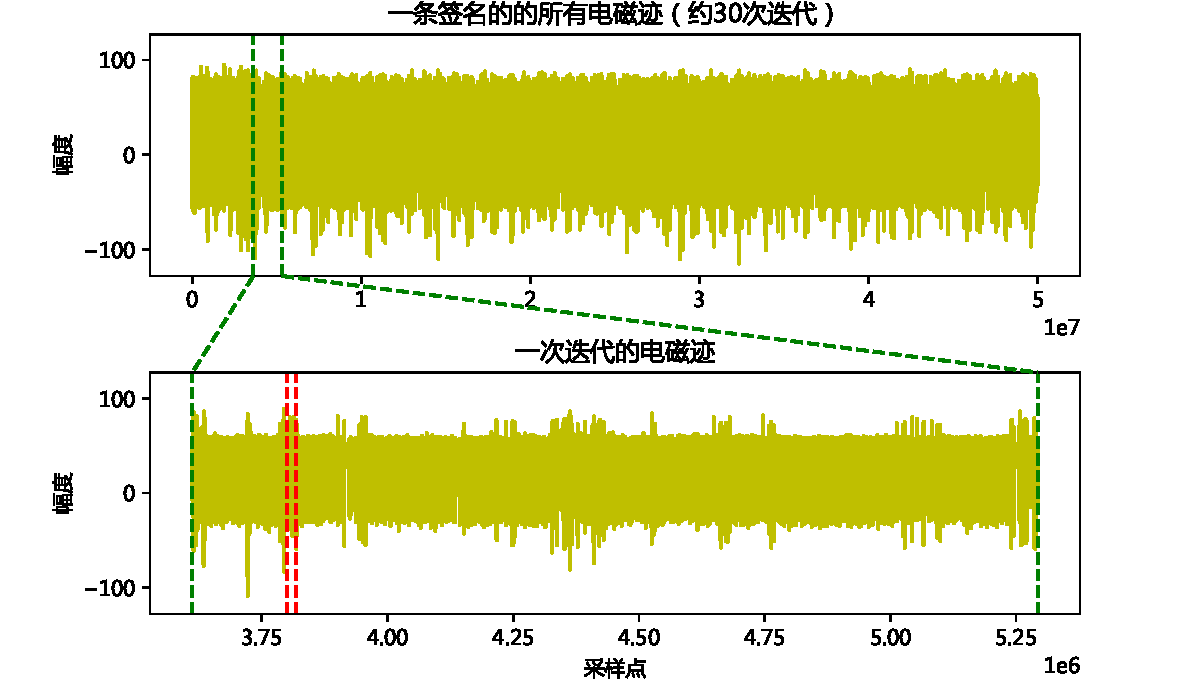
\includegraphics[width=\textwidth]{onetrs}
			\bicaption{\enspace ECDSA实现信息泄漏范围}{\enspace ECDSA Implementation EM Leakage Range}
			\label{fig:onetrs}
		\end{center}
	\end{figure}
	
	%	在阶段一,我们首先对电磁迹分块(对于本研究,第0至359个采样点的所对应的电磁迹的幅度构成第0个块,第360至719个采样点所对应的电磁迹的幅度构成第1个块,以此类推),每块的方差所构成的数列可以与电磁迹相对应,如\figureref{fig:halfphase1}的上、中两幅图所示。从图中可以看到,直观看来电磁迹中较粗的条带(如横坐标为400000附近的区域)所计算出的分块的方差也较大,较细的条带(如横坐标为392000附近的区域)所计算出的分块的方差也较小。这说明分块计算方差考虑到了电磁迹总体的变化趋势,这有助于进一步定位每次迭代的起止位置。
	%	
	%	在计算出每块的方差后,按照阈值执行模数转换和去抖动的操作,去抖动后的数列依然可以与电磁迹相对应,如\figureref{fig:halfphase1}的上、下两幅图所示。从图中可以看到,模数转换和去抖动后的数列所绘制的波形图依然体现了电磁迹总体变化的趋势,并且减小了后续分析的难度(从处理实数数列变为处理01数列)。但是此时的数列依然存在噪声,方波的数量对于每次迭代还是各不相同的,这使得如果仅以此作为辅助信息划分每一次迭代需要让程序频繁进行交叉验证,从而大幅增加时间消耗。
	%	
	%	\begin{figure}[!h]
	%		\begin{center}
	%			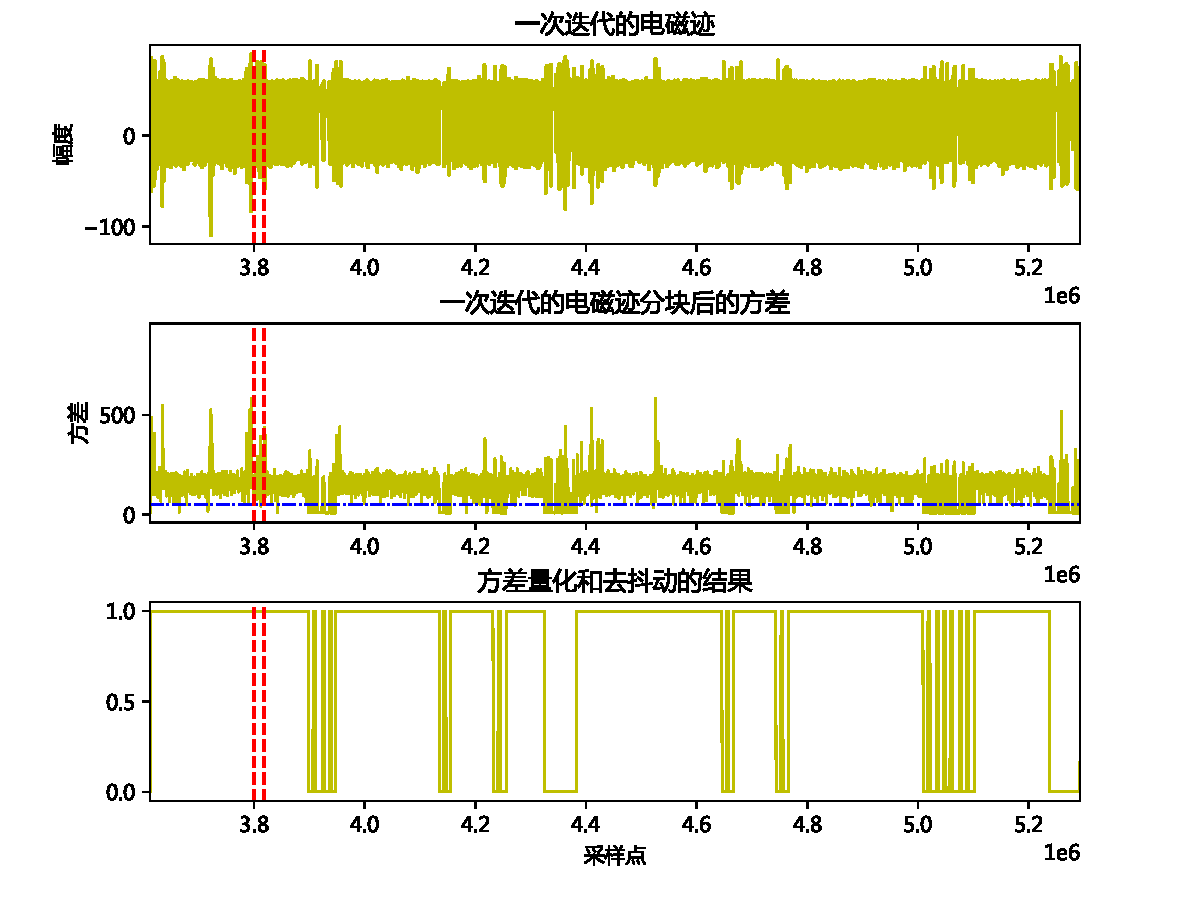
\includegraphics[width=\textwidth]{halfphase1}
	%			\bicaption{\enspace ECDSA实现电磁迹、电磁迹分块后的方差、方差模数转换和去抖动的结果}{\enspace ECDSA Implementation Raw Trace, the Variance of Trace Chunks and the Variance after Quantization and Anti-jitter}
	%			\label{fig:halfphase1}
	%		\end{center}
	%	\end{figure}
	%
	%	为了消除方差模数转换和去抖动的结果中的噪声,我们需要对它做进一步处理。使用模糊函数减小结果中的噪声以及降低层次细节,最终模糊后的数列依然可以与电磁迹相对应,如\figureref{fig:fullphase1}的上、中两幅图所示。从图中可以看到,相比于模糊前,模糊后的数列所绘制的波形图变化更为平缓,偶然的噪声也因为平均了邻域的数值而被减弱。
	%	
	%	在进行模糊后,数列又从01数列变为实数数列,增加了分析的难度。按照新的阈值重新执行模数转换和去抖动的操作,最终的数列还是可以与电磁迹相对应,如\figureref{fig:fullphase1}的上、下两幅图所示。从图中可以看到,模数转换和去抖动仅消除了被模糊所减弱的噪声,减小了后续分析的难度而没有产生其他负面影响。
	%
	随机选取部分计算结果,人工地对标注的信息泄漏范围和在\poifanwei 之后计算出的辅助信息进行对比,如\figureref{fig:fullphase1}所示。\figureref{fig:fullphase1}中红色虚线代表人工标注的敏感信息泄漏范围,绿色虚线代表计算出的辅助信息。比较的内容是每次迭代中人工标注的敏感信息泄漏范围(最右边的红色虚线)与计算出的辅助信息(最左边的绿色虚线)横坐标值之差$\delta$。这些差值的标准差远小于均值,我们有很大的把握(超过99.999\%)认为计算出的辅助信息与随机的横坐标有显著区别。即\poifanwei 有效,可以达到与人工标注同样的效果。
	
	\begin{figure}[!h]
		\begin{center}
			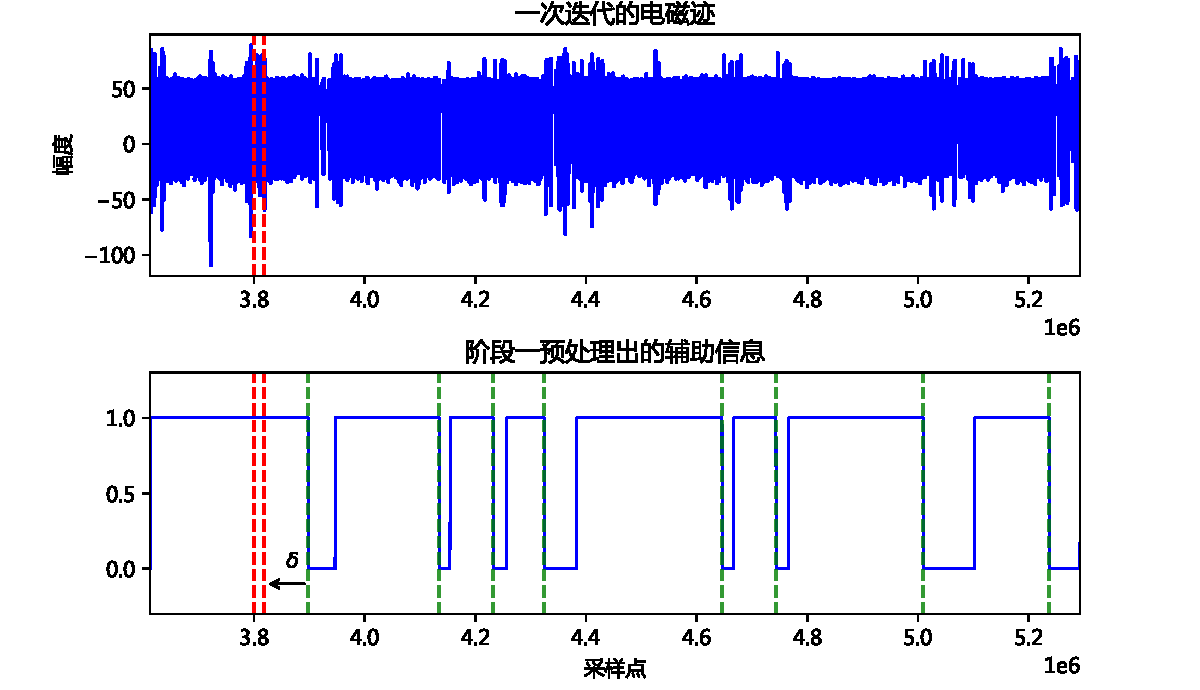
\includegraphics[width=\textwidth]{fullphase1}
			\bicaption{\enspace 计算出的关于电磁子迹的辅助信息}{\enspace Calculated auxiliary information on an EM subtrace}
			\label{fig:fullphase1}
		\end{center}
	\end{figure}
	
	\begin{figure}[!h]
		\begin{center}
			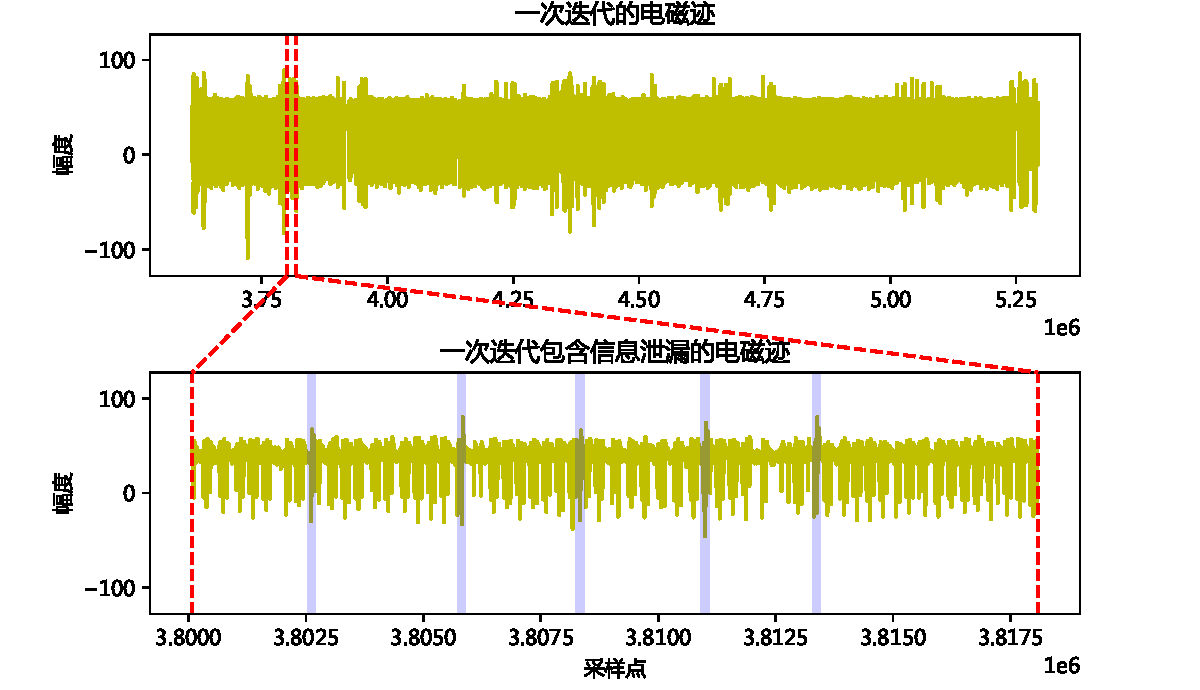
\includegraphics[width=\textwidth]{onetrsleak}
			\bicaption{\enspace 电磁子迹中特征点}{\enspace POIs in an EM subtrace}
			\label{fig:onetrsleak}
		\end{center}
	\end{figure}
	
	%到目前为止,我们可以准确划分出每次迭代,并找出其所对应的电磁迹的泄漏范围,但是还是不能准确确定泄漏位置。
	\figureref{fig:onetrsleak}绘制了所采集到的一条电磁迹在人工标注的泄漏范围内的波形图,其中五处浅蓝色条带是人工标注的POIs。我们期望在\yuchuli 之后可以类似地找到POIs。
{	
	%	使用简单的统计信息难以找到信息泄漏位置。为了解决这个问题,我们使用更复杂的数学工具分析采样点之间内在的联系。我们构造了一个模板,计算模板与所有模板所确定的采样点的邻域各自的协方差作为统计指标用于后续分析。\figureref{fig:rhovscov}展示了使用同一个模板所计算出的协方差与相关系数。从图中可以看到人工标注的信息泄漏位置与相关系数曲线的峰值恰好对应,但是难以和相关系数曲线峰值对应。例如,人工标注的第四处信息泄漏,在协方差曲线的对应位置有显著的峰值,但是在相关系数曲线中对应位置没有特征使得此位置可以从其他假阳性中区分出来。
	%	
	%	\begin{figure}[!h]
	%		\begin{center}
	%			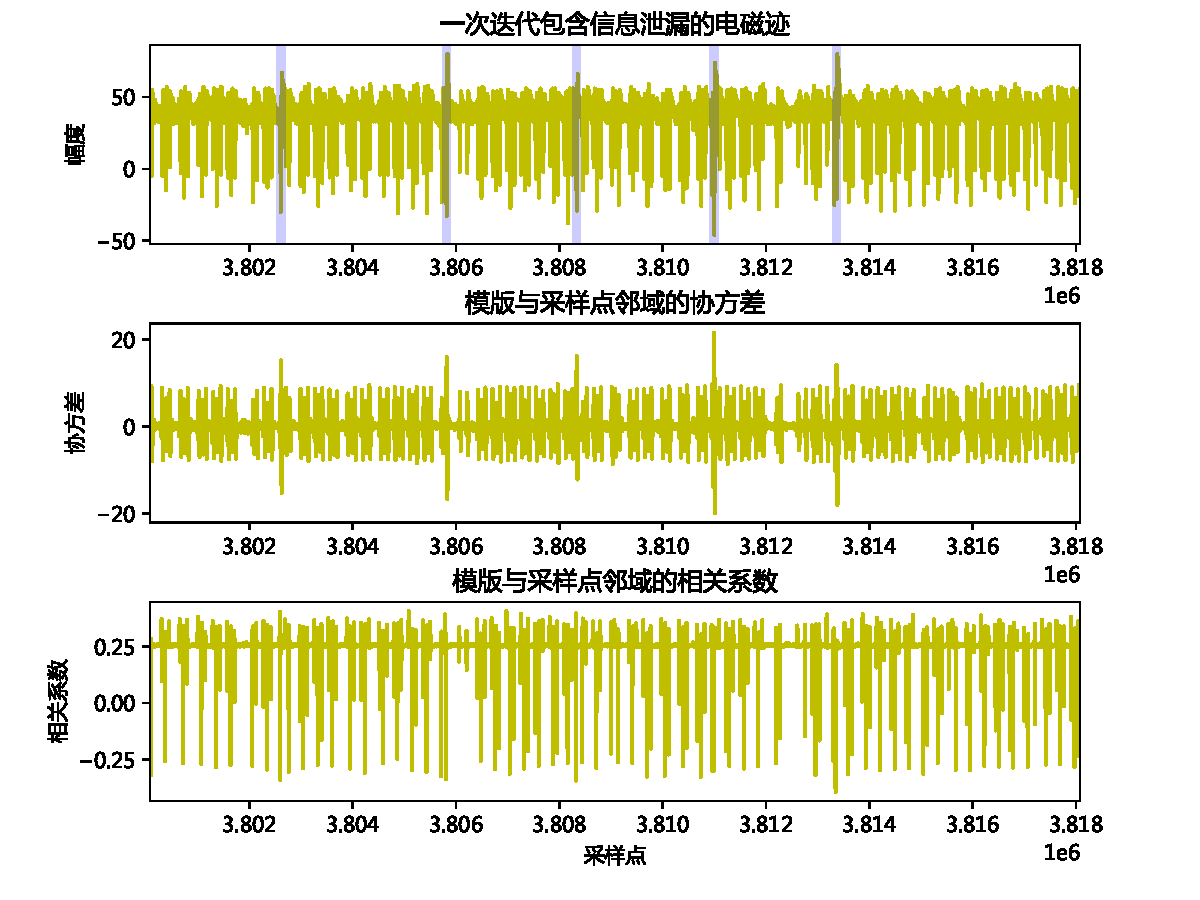
\includegraphics[width=\textwidth]{rhovscov}
	%			\bicaption{\enspace ECDSA实现信息泄漏及其对应的协方差与相关系数}{\enspace ECDSA Implementation EM Leakages and its Corresponding Covariance and Correlation Coefficient}
	%			\label{fig:rhovscov}
	%		\end{center}
	%	\end{figure}
	%
	%	\begin{figure}[!h]
	%		\begin{center}
	%			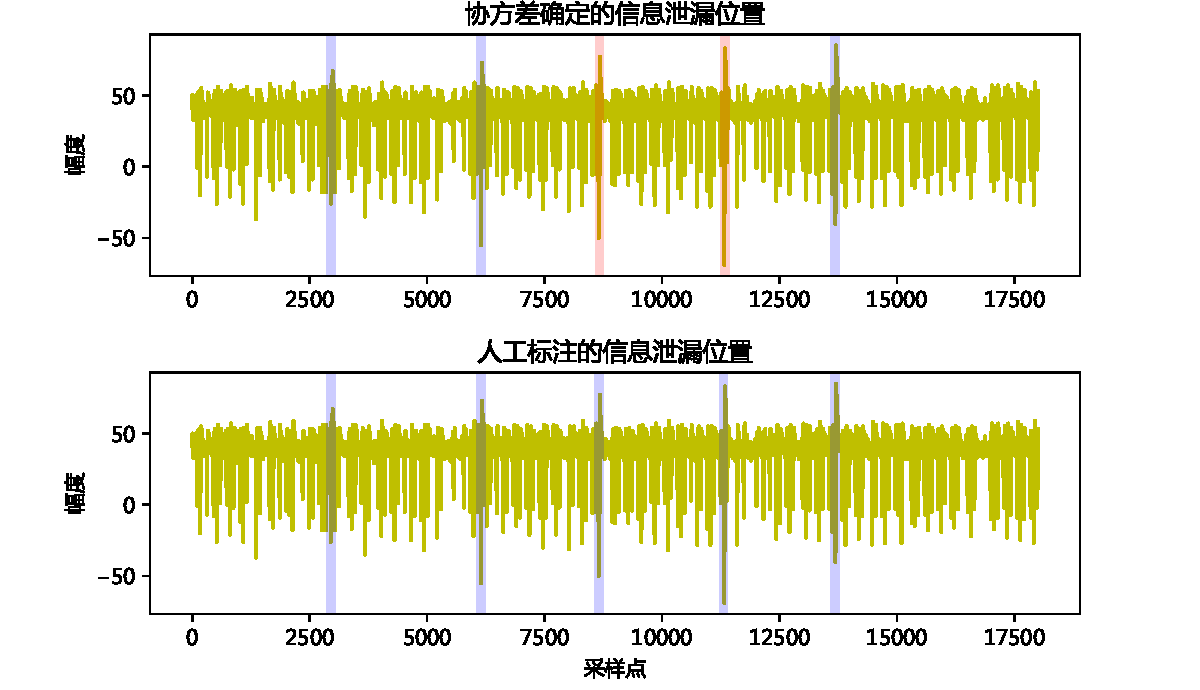
\includegraphics[width=\textwidth]{badmark}
	%			\bicaption{\enspace 计算出的错误信息泄漏位置和标注的信息泄漏位置的差异较小的情况}{\enspace Subtle Differences between Labeled and Wrongly Calculated Leak Positions}
	%			\label{fig:badmark}
	%		\end{center}
	%	\end{figure}
	%	
	%	尽管使用协方差已经帮助找到信息泄漏位置,但是我们在后续研究中发现以此确定的信息泄漏位置可能存在问题,如\figureref{fig:badmark}所示。从图中可以看到,协方差的前5个极值点所确定的信息泄漏位置中,红色条带标注位置是错误的,并不能对应到人工标注的泄漏位置。虽然图中看起来偏差不大,但对应的电磁迹片段和实际信息泄漏完全不符,这会导致后续恢复信息泄漏失败。出现偏差是因为取极值点操作不区分极大值点还是极小值点,从而引入一个系统误差。我们对这种系统误差进行人工统计,在取极值点之后判断是极大值点还是极小值点并据此进行校正,消除系统误差。
	%	
	%	除此之外,有一定信息泄漏存在变形的情况,这使得它对应的协方差并不是前5个极值,而是位于稍微靠后的位置,如第6大的极值(\figureref{fig:badmark2})。本研究尝试后发现,对于所采集的电磁迹,每次迭代取前9个极值点,有超过95\%的概率能找到五个极值点,这五个极值点校正后与人工标注的泄漏位置的几乎重合。
	%	
	%	\begin{figure}[!h]
	%		\begin{center}
	%			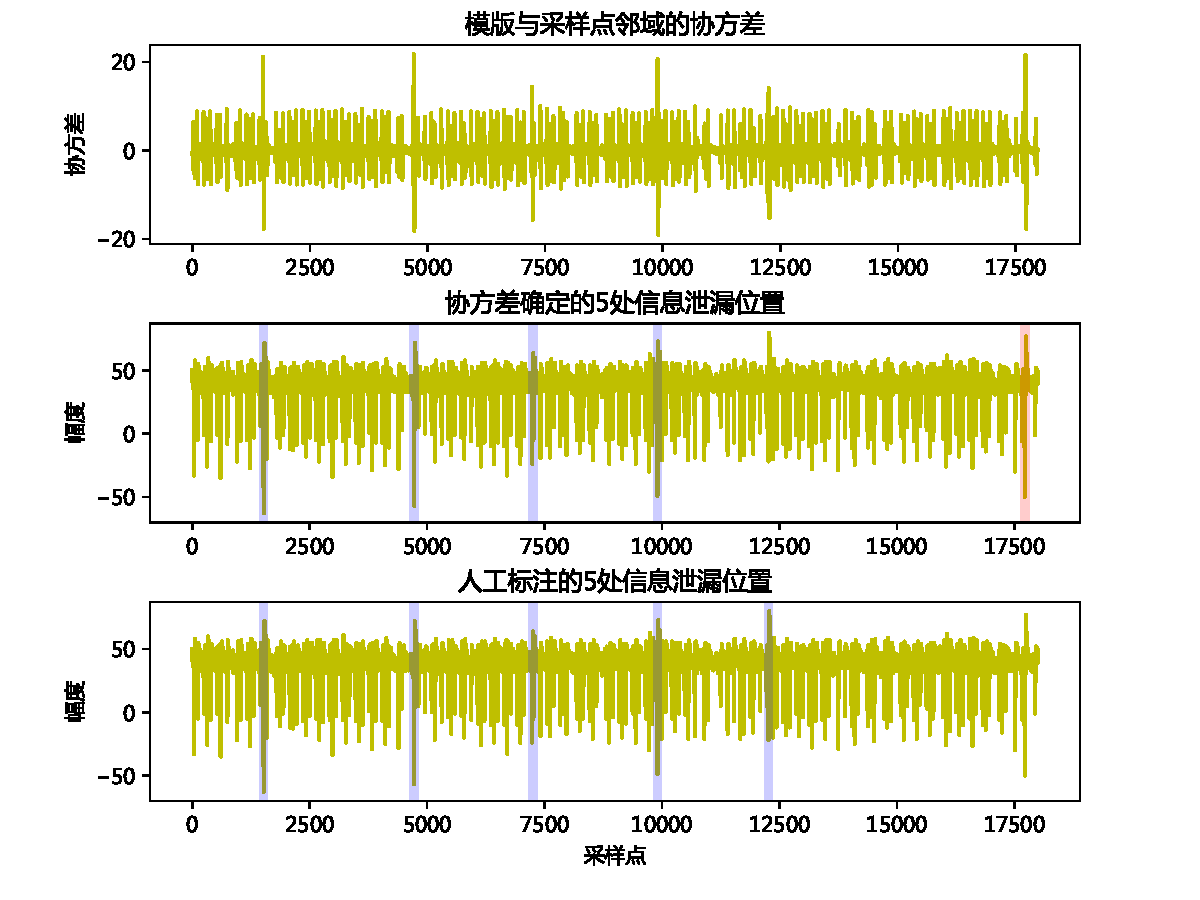
\includegraphics[width=\textwidth]{badmark2}
	%			\bicaption{\enspace 计算出的错误信息泄漏位置和标注的信息泄漏位置的差异较大的情况}{\enspace Substantial Differences between Labeled and Wrongly Calculated Leak Positions}
	%			\label{fig:badmark2}
	%		\end{center}
	%	\end{figure}
	%
	%	为了准确刻画这种重合程度,本文对信息泄漏位置之间采样点的距离建立模板,如\figureref{fig:lambda10}所示。对于一次迭代所对应的多处泄漏,我们认为信息泄漏之间采样点的距离$\delta_0,\delta_1,\dots,\delta_9$应当服从正态分布。\figureref{fig:delta-l0-r1detail}展示了$\delta_0$前1000个样本的概率直方图,从完整的直方图中可以知道,对于大部分迭代所对应的电磁迹,使用协方差找到的第0处信息泄漏位置和第1处信息泄漏位置相隔的采样点个数在3199左右,但是还存在极少数的情况会找错第0处泄漏位置或第1处泄漏位置,这对应于直方图在某些异常的位置(如2516)频数不为0。将数据比较集中的部分进行放大,我们进一步发现直方图可以大致分为三个区间:[3170,3191),[3191,3209)和[3209,3230)。对于区间[3191,3209),它是样本最集中的区域,频数直方图和竖直拉伸后的正态分布曲线(图中蓝色曲线)比较重合,这说明假设$\delta_0$服从正态分布是合理的。另外两个区间不是样本最集中的区域,但是频数直方图也和竖直拉伸后的正态分布曲线(图中黄色、程色曲线)比较重合。实际上,三个区间分别对应这样的情况:
	%	
	%	\begin{itemize}
	%		\item 如果第0处信息泄漏位置是通过协方差取极小值点得出,而第1处信息泄漏位置是通过协方差取极大值点得出,那么这向第0、1处信息泄漏之间采样点的距离中引入了一个小于0的系统误差,$\delta_0$的样本值很可能落在[3170,3191);
	%		\item 如果第0、1处信息泄漏位置通过协方差都取极大值点或都取极小值点得出,这没有向第0、1处信息泄漏之间采样点的距离引入系统误差,那么$\delta_0$的样本值很可能落在[3191,3209);
	%		\item 如果第0处信息泄漏位置是通过协方差取极大值点得出,而第1处信息泄漏位置是通过协方差取极小值点得出,那么这向第0、1处信息泄漏之间采样点的距离中引入了一个大于0的系统误差,$\delta_0$样本值很可能落在[3209,3230)。
	%	\end{itemize}
	%
	%	这进一步说明取极值点操作应当区分极大值点还是极小值点并及时校正,从而避免系统误差。校正之后,频数直方图数据分布变得更集中了。对于$\delta_1,\delta_2,\dots,\delta_9$,他们的情况和$\delta_0$类似,唯一不同之处在于正态分布的均值和方差一般是不同的,如\appfigureref{appfig:deltaall}所示,因此总共需要计算10次时间的模板。
	%	
	%	%视为我们人工对少量(10条电磁迹合计约300次迭代)电磁迹的信息泄漏位置进行标注,统计这些位置之间的差值的均值和方差,作为刻画重合程度的模板。
	%	
	%	\begin{figure}[!h]
	%		\begin{center}
	%			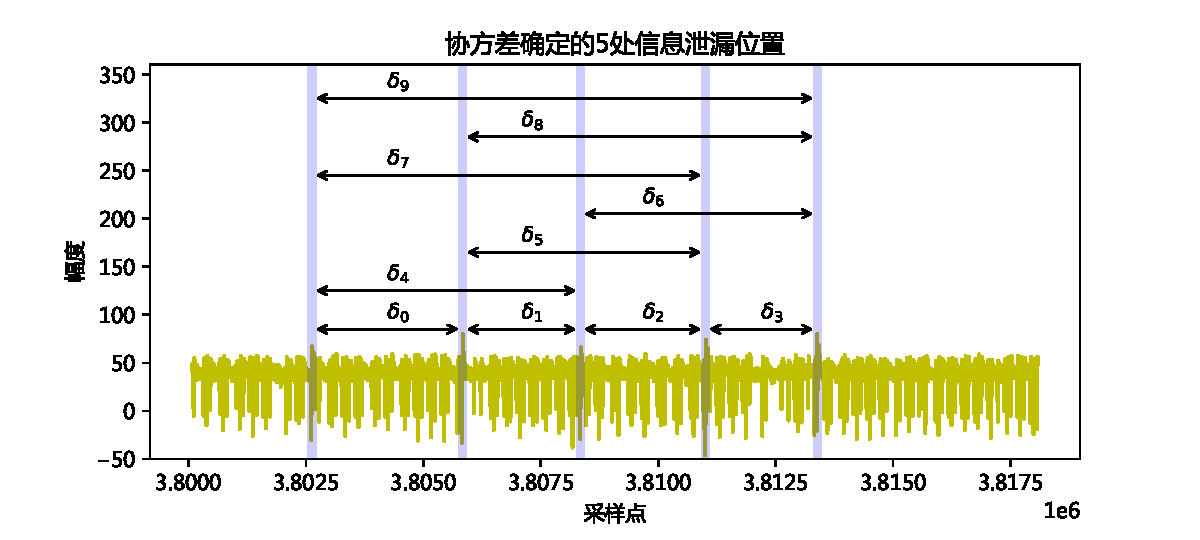
\includegraphics[width=\textwidth]{lambda10}
	%			\bicaption{\enspace 信息泄漏位置之间的距离示意图}{\enspace Demostration of Calculating Distance between Leak Positions}
	%			\label{fig:lambda10}
	%		\end{center}
	%	\end{figure}
	%	
	%	\begin{figure}[!h]
	%		\begin{center}
	%			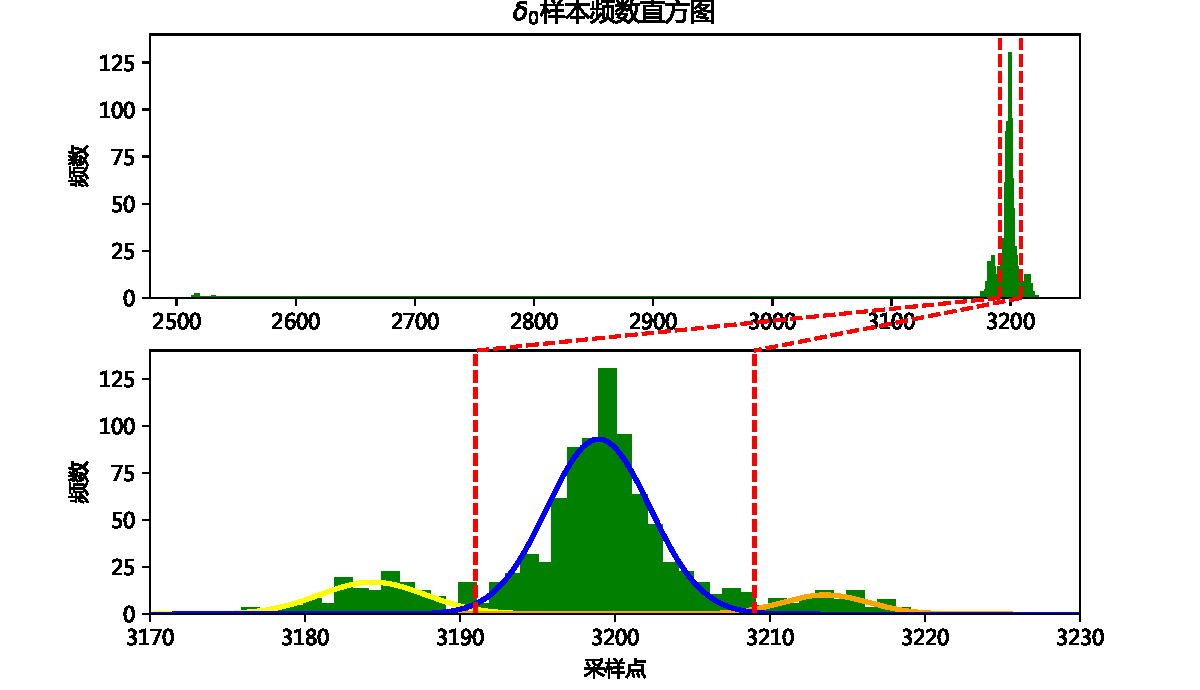
\includegraphics[width=\textwidth]{delta-l0-r1detail}
	%			\bicaption{\enspace 1000个$\delta_0$的样本频数直方图}{\enspace Frequency Histogram of 1000 $\delta_0$ Samples}
	%			\label{fig:delta-l0-r1detail}
	%		\end{center}
	%	\end{figure}
	%
	%	使用校正后的前9个极值点以及预计算的模板,\algorithmref{alg:checkdelta}可以筛选出符合模板的极值点,进而确定信息泄漏位置,如\figureref{fig:select9}所示。虽然前9个极值点中一定会有错误的,但是进行模板检查之后可以排除这种错误,从而准确选出理论上会对应信息泄漏的5个极值点。在极少的情况下(占所有情况的比例少于5\%),找不到符合模板的极值点,因此无法确定某一次迭代的信息泄漏位置,也就无法恢复此次迭代的信息泄漏。需要注意的是,这种情况不会直接导致攻击失败,只是会增加找到可利用(连续4比特)的敏感信息泄漏的难度。
	%	
	%	\begin{figure}[!h]
	%		\begin{center}
	%			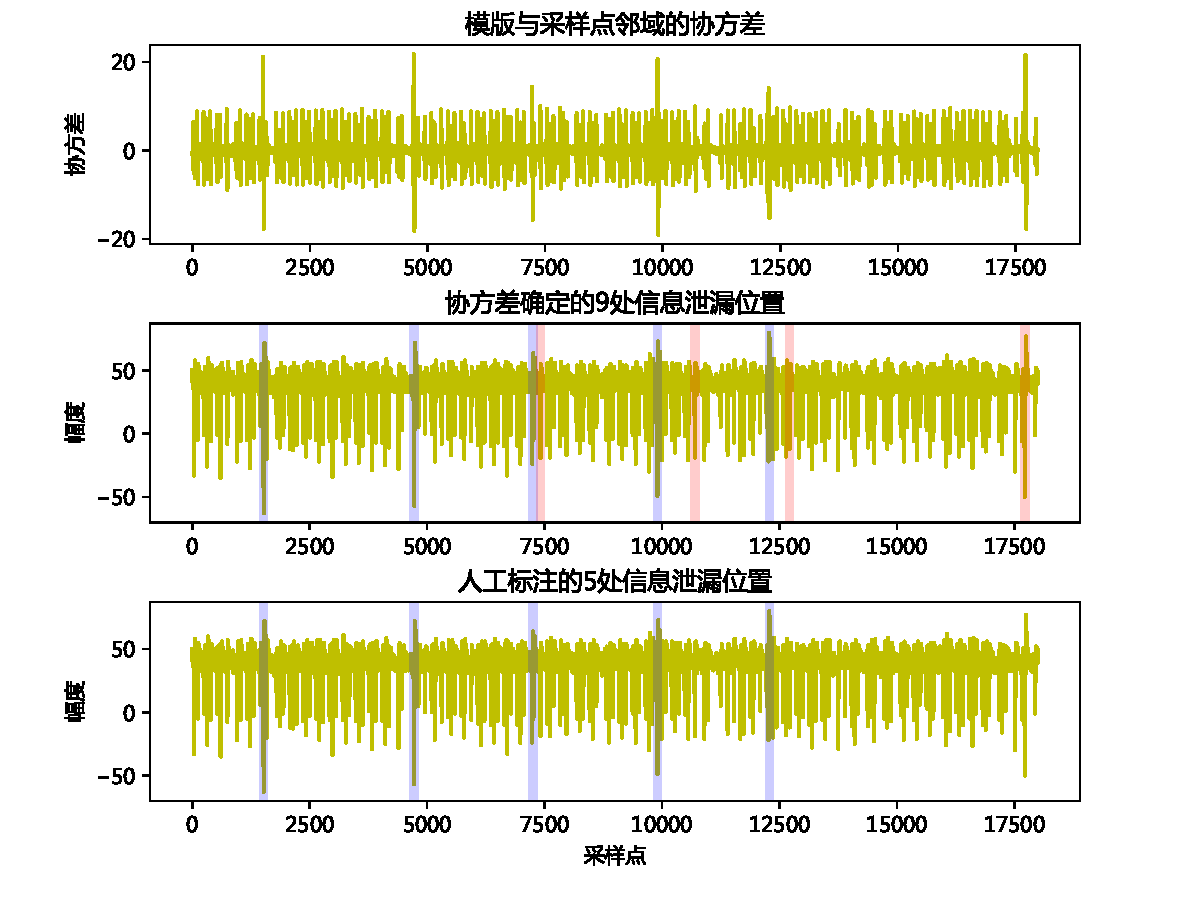
\includegraphics[width=\textwidth]{select9}
	%			\bicaption{\enspace 协方差极值点不能确定的信息泄漏位置的情况}{\enspace Failing to Determine the Leak Position using Argmax of Covariance}
	%			\label{fig:select9}
	%		\end{center}
	%	\end{figure}
}

	随机选取部分计算结果,人工地对标注的POIs和在\yuchuli 之后计算出的POIs进行对比。对比的方法是,根据POIs对电磁子迹进行对齐,量化评价电磁子迹的对齐程度可以从侧面发型POIs提取的准确程度。
	获得了POIs后,我们从相应位置及其邻域\footnote{邻域的大小可以自行设定。在本研究中,邻域设定为以当前位置为中心,左右各150个采样点的区间。}提取电磁子迹并重新对采样点编号。\figureref{fig:aligndemo}绘制了提取出的每次迭代的第二处包含信息泄漏的电磁子迹,上图是500条中间值$\tilde\nonce_j=1$的电磁迹以及500条中间值$\tilde\nonce_j=3$的电磁迹,下图是这1000条能量迹进行TVLA的结果。下图TVLA结果在第140个采样点取得极值且超过阈值4.5,因此提取出的电磁子迹在第140个采样点处对齐且存在敏感信息泄漏的置信水平达到99.999\%。上图中曲线的颜色的深浅可以体现某一类能量迹的集中程度,可以看出,$\tilde\nonce_j=1$所对应的电磁迹在第140个采样点的幅度总体来说是比$\tilde\nonce_j=3$所对应的幅度大,这与TVLA的结果是一致的。根据结果认为\yuchuli 达到了预期效果,可以准确确定POIs,也能在此基础上进行电磁子迹的对齐。对于每次迭代包含敏感信息泄漏的电磁迹,不同中间值$\tilde\nonce_i$之间TVLA结果见\appfigureref{appfig:aligndemoall}。
	
	\begin{figure}[!h]
		\begin{center}
			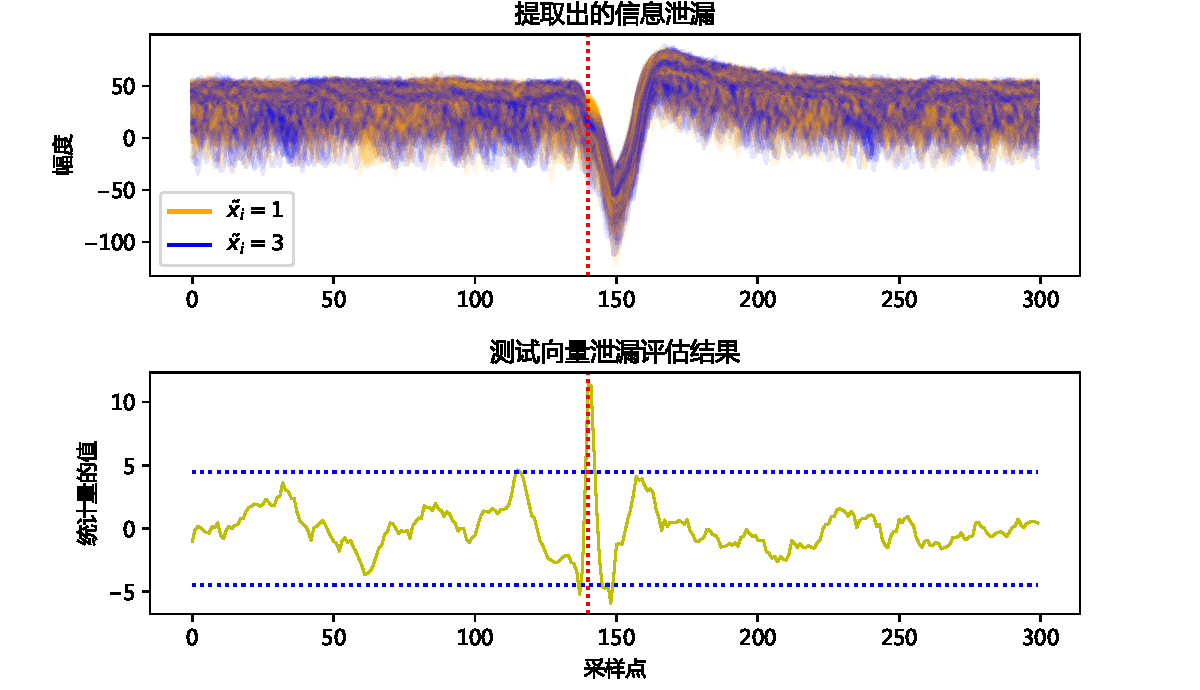
\includegraphics[width=\textwidth]{aligndemo}
			\bicaption{\enspace 每次迭代包含第二处信息泄漏的电磁子迹及其TVLA结果}{\enspace Subtraces Containing the Second Leakage and their TVLA Result}
			\label{fig:aligndemo}
		\end{center}
	\end{figure}

{	
	%	在评估阶段,我们只能知道每个$\tilde \nonce_i$的值但是不能准确知道每个$\leakedmultiplier_i$的值,如\tableref{tab:partialknownti}所示。我们从所有迭代含有信息泄漏的电磁迹中过滤出了对应的$\leakedmultiplier_i$完全确定的电磁迹(即从所有电磁迹中只选出对应的$\tilde \nonce_i\neq0$的电磁迹)并使用TVLA进行泄漏检测。对于每次迭代包含其它信息泄漏的电磁迹,不同中间值$\leakedmultiplier_i$之间TVLA结果见\appfigureref{appfig:aligndemoall}。
	%	
	%	\begin{table}[!htb]
	%		\bicaption{\enspace 评估时可以推断的$\leakedmultiplier_i$的信息}{\enspace Deduced $\leakedmultiplier_i$ for Evaluation}
	%		\label{tab:partialknownti}
	%		\centering
	%		\begin{subtable}{\twof\textwidth}
	%			\centering
	%			\begin{tabular}{cc|ccc}
	%				\hline
	%				\multicolumn{2}{c|}{\multirow{2}{*}{$\Pr[\leakedmultiplier_i=v|\tilde \nonce_i=w]$}} & \multicolumn{3}{c}{$v$} \\
	%				%\cline{3-5}
	%				\multicolumn{2}{c|}{}& 1 & 2 & 3 \\
	%				\hline
	%				\multirow{4}{*}{$w$} & 0 & $\frac12$ & $\frac14$ & $\frac14$ \\
	%				%\cline{2-5}
	%				& 1 & 1 & 0 & 0 \\
	%				%\cline{2-5}
	%				& 2 & 0 & 1 & 0 \\
	%				%\cline{2-5}
	%				& 3 & 0 & 0 & 1 \\
	%				\hline
	%			\end{tabular}
	%			\subcaption{$\leakedmultiplier_i$的条件分布列}
	%			\label{tab:partialknowntidetail}
	%		\end{subtable}\hfill
	%		\begin{subtable}{\twof\textwidth}
	%			\centering
	%			\begin{tabular}{c|cc}
	%				\hline
	%				$\tilde \nonce_i$数值&能否知道$\leakedmultiplier_i$数值&$\leakedmultiplier_i$数值\\
	%				\hline
	%				0 & 否 & /\\
	%				1 & 是 & 1\\
	%				2 & 是 & 2\\
	%				3 & 是 & 3\\
	%				\hline
	%			\end{tabular}
	%			\subcaption{由$\tilde \nonce_i$可以推断的$\leakedmultiplier_i$的信息}
	%			\label{tab:partialknownticonclusion}
	%		\end{subtable}
	%	\end{table}
	%
	%	总的来说,进行阶段二之后我们可以成功提取包含信息泄漏的电磁迹且能通过TVLA检测出存在信息泄漏。经过阶段一和阶段二,提取出包含信息泄漏的电磁迹后,还需要从中恢复信息泄漏才能完成对智能卡ECDSA实现的侧信道分析整个流程。
}

	\subsection{未采用数据增强的模板构建}
	\algorithmref{alg:filter}会输出五个数据集,使用任何一个可以获得的效果是类似的。实验发现在仅使用一组电磁子迹的情况下使用$L_1^{out}$可以获得最优的结果,因此后续只列举利用$L_1^{out}$和$Label^{out}$进行建模和攻击的结果。提取POIs并构造数据集后,将$cnt\approx100000$个样本拆分为5组,每组20000个样本(舍去剩余的)。这么做的原因是可以对于同一张双界面商用智能卡所采集的电磁迹,构造出的数据集可以进行互相独立的五次实验。每一组又拆分为训练集、验证集和测试集,大小分别设置为10000、5000、5000。本研究中训练集设置相比于通常训练集的占比80\%较少有两个原因,一个是训练深度学习模型的数据增强后的训练集而数据增强后的训练集会比数据增强前更大,另一个原因是这样可以使得通用数据增强方法对DL-SCA提升的效果更明显。
	
	深度学习模型的超参数与\subsref{subs:useagmt}中深度学习模型设置一致。
	
	一组样本只进行一次实验,5组样本总共进行5组实验,最后的结果取五组中的最优。取最优的原因有两个,一个是在现实场景中攻击只用成功一次就说明攻击目标存在漏洞,另一个在大部分情况下是恢复私钥的时间只能在理论上进行估计而不能实际计算。
	
	在未采用数据增强方法时,DL-SCA使用$L_1^{out}$进行训练和验证的结果如\figureref{fig:ecdsanoda}所示。从图中可以看出随着训练轮次逐渐增加,验证集精确率逐渐提升,说明训练有效。在训练完成后,测试集精确率(使用极大似然估计时的真阳性率,见\subsref{subs:useagmt}中\textbf{攻击评估单元设置}部分。)可以达到91.35\%。%,在这种情况下,运用格方法恢复双界面商用智能卡ECDSA私钥的时间在理论上会超过七百万年。
	
	在特征点提取之后,电磁迹的采样点个数从50000000减小为300\footnote{$150*2=300$它表示邻域设定为以一个特征点为中心,左右各150个采样点的区间。},深度学习模型的所占用的存储空间变为原来的$\frac{3}{500000}$。数据处理前深度学习训练阶段会使用167条电磁迹训练20个训练轮次,计算量为$8.7\cdot10^{16}$浮点运算次数(Floating Point Operation,FLOP)。提取特征点构造新的数据集后深度学习训练阶段会使用5000条电磁子迹(167条电磁迹包含共5010次迭代的敏感信息泄漏,这对应于5010条电磁子迹)训练20个训练轮次,计算量减少为$1.6\cdot10^{13}$FLOPs。对本研究的实验环境而言,算力不超过3.2G\footnote{实际上CPU主频为3.2GHz,算力难以直接测量。在不考虑数据并行的情况下,CPU每个时钟周期执行最多一次浮点运算,此时算力数值大小不超过CPU主频数值大小。}每秒浮点运算次数,因此深度学习训练阶段所消耗的时间会从315天减小为8分钟。实际实验中,DL-SCA时间为490秒(8分10秒),与理论分析一致。%样本数量变为原来的30倍,因此深度学习模型训练阶段计算量减小为原来的$\frac{9}{50000}$。
	
	\begin{figure}[!h]
		\centering
		\begin{subfigure}[b]{\twof\textwidth}
			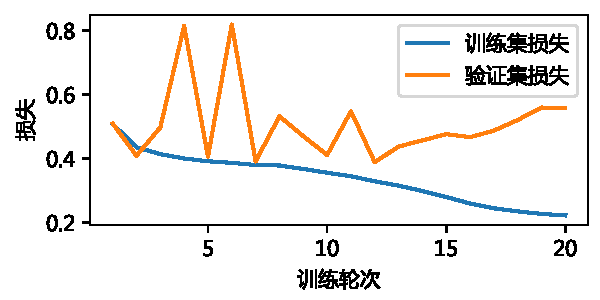
\includegraphics[width=\textwidth]{ecdsanodaloss}
			\caption{负对数交叉熵损失}
			\label{fig:ecdsanodaloss}
		\end{subfigure}%
		~% add desired spacing
		\begin{subfigure}[b]{\twof\textwidth}
			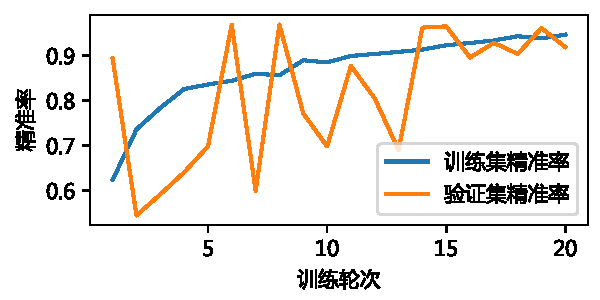
\includegraphics[width=\textwidth]{ecdsanodaprecision}
			\caption{精确率}
			\label{fig:ecdsanodaprecision}
		\end{subfigure}
		\\
		\bicaption{\enspace 无数据增强的DL-SCA训练和验证结果}{\enspace Training and validation results of DL-SCA without DA}
		\label{fig:ecdsanoda}
	\end{figure}

	\subsection{\shujuzengqiang}
	
	采用面向基于深度学习侧信道分析的数据增强方法后,DL-SCA使用$L_1^{out}$进行训练和验证的结果如\figureref{fig:ecdsaada}所示。在训练完成后,测试集精确率(使用极大似然估计时的真阳性率)可以达到95.50\%。%,在这种情况下,运用格方法恢复双界面商用智能卡ECDSA私钥的时间在理论上会达到12.5年。
	采用数据增强方法会导致DL-SCA时间由8分钟增长到1小时,还额外引入2分钟的数据增强时间,但是对于格方法减少的时间而言,所增加的时间可以忽略不计。
	
	\begin{figure}[!h]
		\centering
		\begin{subfigure}[b]{\twof\textwidth}
			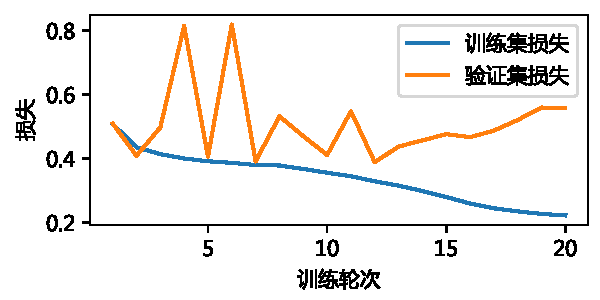
\includegraphics[width=\textwidth]{ecdsanodaloss}
			\caption{负对数交叉熵损失}
			\label{fig:ecdsaadaloss}
		\end{subfigure}%
		~% add desired spacing
		\begin{subfigure}[b]{\twof\textwidth}
			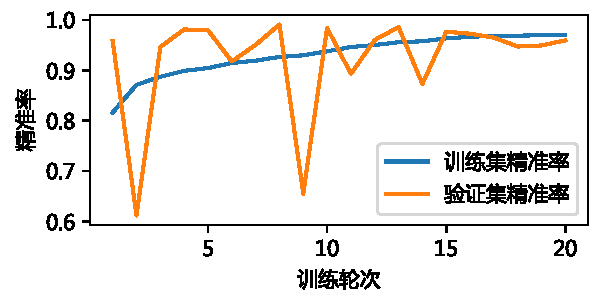
\includegraphics[width=\textwidth]{ecdsaadaprecision}
			\caption{精确率}
			\label{fig:ecdsaadaprecision}
		\end{subfigure}
		\\
		\bicaption{\enspace 采用通用数据增强方法的DL-SCA训练和验证结果}{\enspace Training and validation results of DL-SCA with general DA method}
		\label{fig:ecdsaada}
	\end{figure}

	\subsection{\jiashejianyanguji}
	采用\jiashejianyanguji 方案后,DL-SCA使用$L_1^{out}$进行训练和验证的结果如\figureref{fig:ecdsatpr}所示。可以看出,无论是否采用数据增强方法,提高显著水平$\alpha$可以提高真阳性率。在训练完成后,在显著水平$\alpha=0.51056$、使用本研究采集的数据、独立进行5次进行深度学习模型的训练和测试、每次使用5000条电磁子迹进行测试的情况下,测试集真阳性率都达到100\%。%在这种情况下,理论上运用格方法可以恢复双界面商用智能卡ECDSA私钥,平均时间为400秒。
	
	
	\begin{figure}[!h]
		\centering
		\begin{subfigure}[b]{\twof\textwidth}
			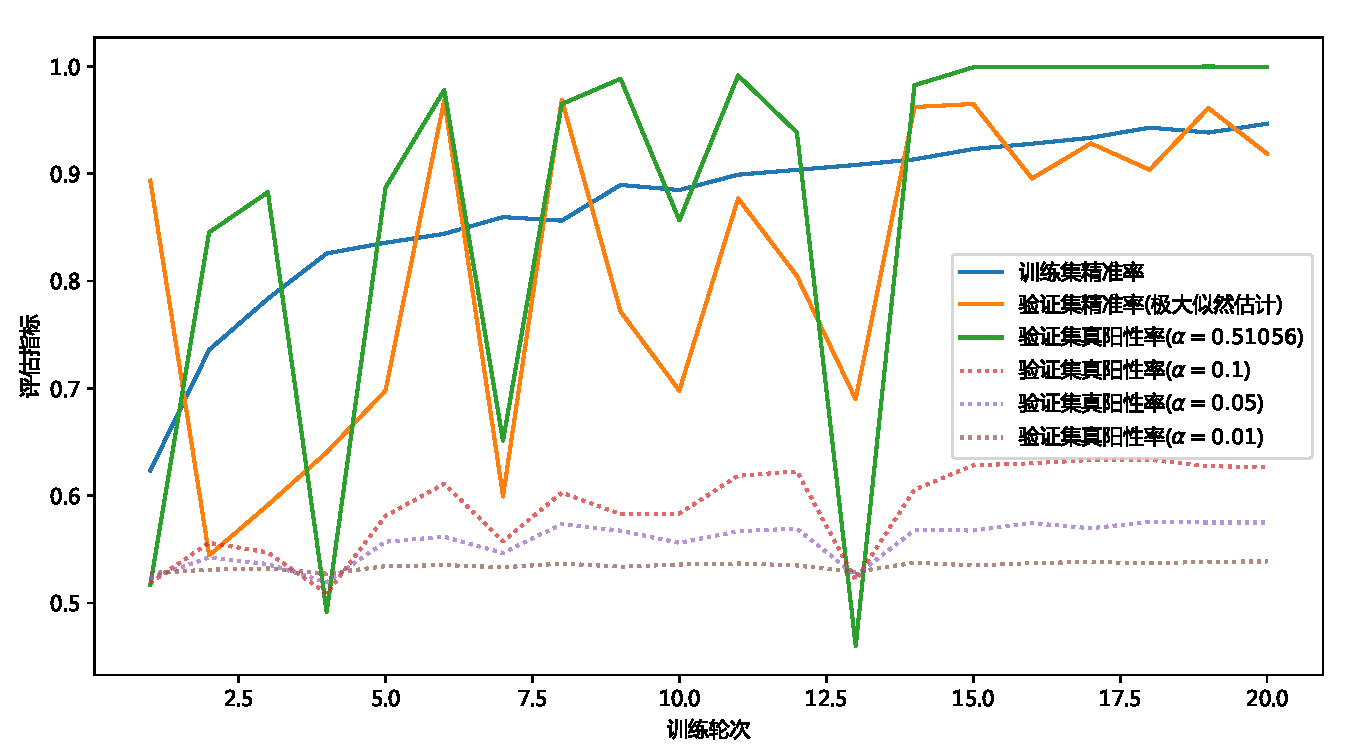
\includegraphics[width=\textwidth]{ecdsanodatpr}
			\caption{未采用数据增强}
			\label{fig:ecdsanodatpr}
		\end{subfigure}%
		~% add desired spacing
		\begin{subfigure}[b]{\twof\textwidth}
			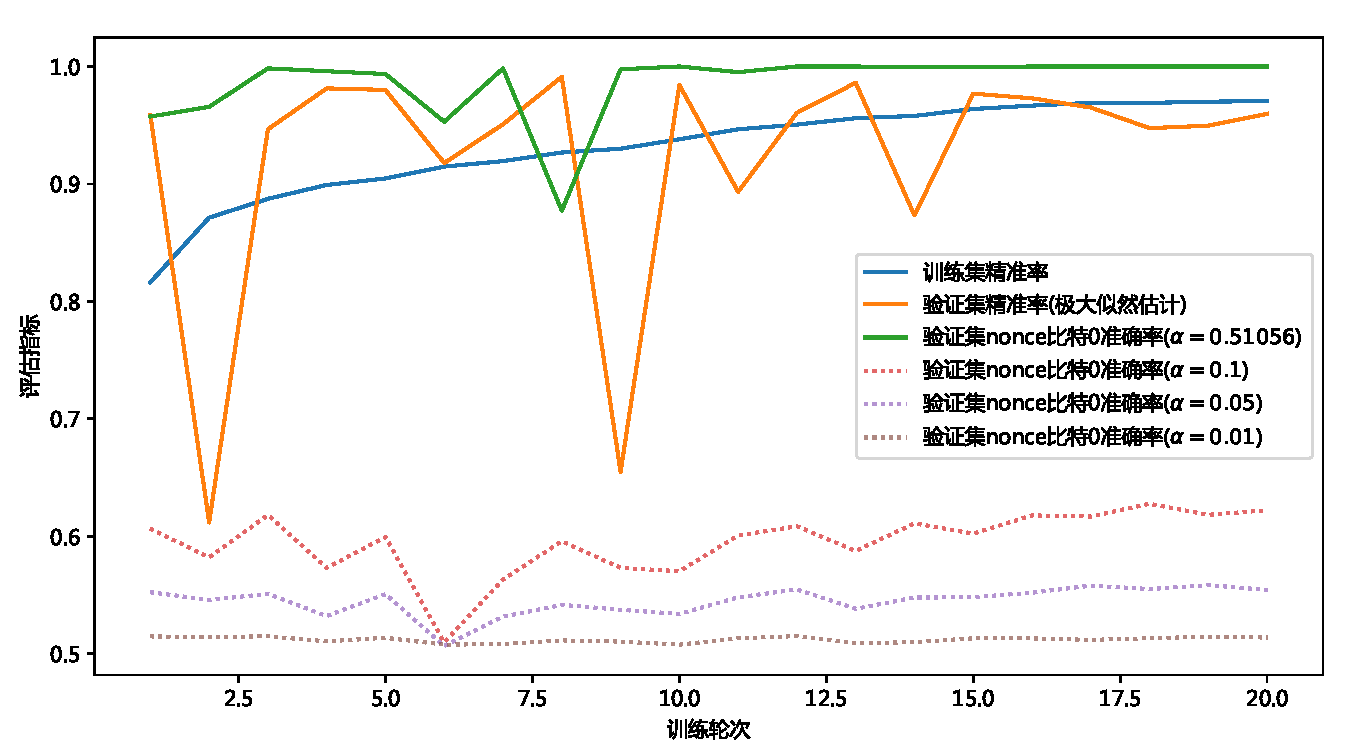
\includegraphics[width=\textwidth]{ecdsaadatpr}
			\caption{采用数据增强}
			\label{fig:ecdsaadatpr}
		\end{subfigure}
		\\
		\bicaption{\enspace DL-SCA训练和验证结果}{\enspace Training and validation results of DL-SCA}
		\label{fig:ecdsatpr}
	\end{figure}
	
	
	\subsection{采用电磁分析的后续效果}
	{\color{\xchange}
	
	\tableref{tab:improve}列举了本方法在型号为J3D081的Java卡进行电磁分析验证以及Roche等\citep{Roche21}在谷歌安全产品\textit{Google Titan Security Key}\citep{Titan}进行攻击的结果。两个研究对象使用了相同的安全微控制器芯片SmartMX\citep{p5x}。%暴力破解是逐一枚举$Z_q$中所有元素并逐一进行验证的方法,它描述了攻击密码算法时的最坏情况。Zaid等\citep{Zaid20}针对ASCADf(N=50)数据集设计的深度神经网络,调整网络输入为50000000,训练轮次为20之后理论上讲可以进行电磁分析攻击。
	Roche等\citep{Roche21}他们运用了滤波的预处理技术、聚类以及格方法实施攻击。本研究运用了\yuchuli 预处理技术、面向基于深度学习侧信道分析的通用数据增强方法、\jiashejianyanguji 方案以及格方法实施攻击。
	
	\begin{table}[!h]
		\bicaption{\enspace 采用工作的效果}{\enspace Nuts to crack in attacking the smart card}
		\label{tab:improve}
		\centering
		\tiny% fontsize
		%\setlength{\tabcolsep}{4pt}% column separation
		%\renewcommand{\arraystretch}{1.2}%row space 
		\begin{tabular}{c|cccccc}
			\hline
			工作&采集时间&预处理时间&数据增强时间&DL-SCA时间&聚类时间&真阳性率\\
			\hline
			Roche等\citep{Roche21}&6小时&/&0&0&/&99.6\%\\
			本研究&1天&3天&2分钟&1小时&0&100\%\\
			\hline
		\end{tabular}
		\tabnote{数据不详使用斜杠/ 标记。}
	\end{table}

	%从可计算性的角度来看,枚举空间$q\approx2^{256}$(椭圆曲线$E$的阶)是个有限的数,使用暴力破解足以恢复ECDSA私钥。就本研究的实验环境(处理器型号为Intel(R) Xeon(R) CPU E5-2667 v4 @ 3.20GHz,内存大小252GB)而言,枚举100000个元素并逐一验证需要约7秒。因此枚举$q$个元素进行暴力破解最坏需要$2.6\times10^{65}$年,平均需要$1.3\times10^{65}$年,这在现实中是难以接受的。暴力破解没有改进的空间,因此实际需要使用其他攻击思路,例如尝试使用侧信道分析恢复私钥。
	
	%将Zaid等\citep{Zaid20}的深度学习网络套用到侧信道分析的现实场景,理论可行但是实际存在时间开销长的问题。这也导致就本研究的实验环境,无法计算准确的真阳性率,从而无法估计使用格方法所需要的时间。
	
	Roche等\citep{Roche21}等与本研究的主要不同之处在于他们使用聚类的方法恢复敏感信息泄漏,真阳性率可达到99.6\%。恢复敏感信息泄漏后,他们使用了数十次\footnote{原文如此:few tens of attempts。}格方法才成功求解私钥,每次运用格方法在他们的实验环境下(3.3GHz Intel Core i7, 16GB RAM)需要约100秒\footnote{原文如此:about 100 seconds to complete。}。
	
	%尽管直接套用Zaid等\citep{Zaid20}提出的DL-SCA存在时间开销长的问题,但是这项技术存在很大的改进空间。本研究就是在其提出的深度学习模型上加以改进,最终完成了侧信道分析。
	%本研究提出并使用\yuchuli 预处理技术,以增加预处理时间作为代价,显著降低了执行DL-SCA的时间。本研究使用\chapref{chap:search1}的数据增强方法,以增加数据增强时间和DL-SCA时间作为代价,提高了真阳性率。最后,本研究利用格方法攻击目标双界面商用智能卡ECDSA实现的特点(对敏感信息泄漏估计值假阳性敏感,假阴性不敏感)提出并使用\jiashejianyanguji 方案,进一步提高真阳性率,达到100\%。
	
	本研究使用深度学习作为主体进行电磁分析。在深度学习的基础上,使用\yuchuli 预处理技术、面向基于深度学习侧信道分析的数据增强方法、\jiashejianyanguji 方案将深度学习模型的真阳性率提升到100\%,减少运用格方法恢复私钥的时间。就运用格方法的时间而言,本研究实验环境下((处理器型号为Intel(R) Xeon(R) CPU E5-2667 v4 @ 3.20GHz,内存大小252GB)为400秒,低于Roche等\citep{Roche21}约几千秒的结果。
	
	除此之外,Roche等\citep{Roche21}采集了6000条电磁迹,理论上可以划分出768000条电磁子迹用于电磁分析。本研究仅采集5000条电磁迹,划分出100000条电磁子迹用于电磁分析。本研究在使用更少的数据达到了更优的技术效果。
	
	%就攻击时间而言,本研究与Roche等\citep{Roche21}在研究对象、攻击方法等方面最为相似。\tableref{tab:improve}中数据显示本研究的攻击时间长于Roche等\citep{Roche21}的攻击时间,这是因为实验环境(例如采集电磁迹的示波器、电脑算力)存在差异、Roche等\citep{Roche21}未汇报所使用的滤波的预处理技术以及格方法的细节和时间开销。
	}

	\section{本章小结}
	{\color{\xchange}
	
%	对本研究而言,侧信道分析需要在有限计算资源下,在可接受的时间范围内结合格方法恢复双界面商用智能卡ECDSA私钥。
%	
%	针对DL-SCA时间长、运用格方法时间长这两个直接问题,本研究提出并使用\yuchuli 预处理技术、面向基于深度学习侧信道分析的数据增强方法以及\jiashejianyanguji 方案,将成功恢复ECDSA私钥的时间从理论上约$2\times10^{85}$年减小到4天,完成了针对目标双界面商用智能卡的分析。
	本研究提出了面向双界面商用智能卡ECDSA实现的电磁分析方法,并给出了参考实现。该方法可以恢复型号为J3D081的Java卡的ECDSA实现敏感信息泄漏,并在与格方法结合时恢复ECDSA私钥。实际应用时,本研究在1天内采集5000条电磁迹、3天内进行电磁迹预处理得到样本数量为100000数据集、137秒内对数据集中的训练集进行数据增强、1小时内实施DL-SCA恢复敏感信息泄漏。电磁分析后可以从5000条电磁迹对应的的签名中,过滤出119条可以被后续格方法所利用的含有连续4比特敏感信息泄漏的签名,多于75条。这119条签名含有的连续4比特敏感信息泄漏都正确。达到了后续使用由敏感信息泄漏恢复私钥的格方法的必要条件。
	
	本研究使用了\yuchuli 技术。它通过\poifanwei 技术将特征点范围从50000000缩小到18000,接着使用相关系数极值点的时间模板实现特征点提取,执行TVLA后可以检测出泄漏。提取特征点后,还完成了电磁迹的预处理,成功构造了用于深度学习的数据集。
	
	本研究使用了\shujuzengqiang。它选择最优的数据增强策略参数对现有数据集中的训练集进行数据增强,使得实际攻击时在不额外采集电磁迹的情况下将DL-SCA的真阳性率由91.35\%提高到95.50\%。
	
	本研究使用了\jiashejianyanguji。它利用格方法攻击目标双界面商用智能卡ECDSA实现的特点(对敏感信息泄漏估计值假阳性敏感,假阴性不敏感),通过使用更严格的标准估计阳性样本。在显著水平$\alpha=0.51056$、使用本研究采集的数据、独立进行5次进行深度学习模型的训练和测试、每次使用5000条电磁子迹进行测试的前提下,真阳性率都达到100\%。
	
	这个参考实现为密码评估和设计人员提供了便捷、高效的面向双界面商用智能卡的电磁分析方法。这个高效的电磁分析方法可以提高攻击依赖型侧信道安全检测的准确性和可靠性,有助于改善和提升智能卡信息泄漏分析和物理安全性测评的技术能力,对建立先进的智能卡物理安全性评估体系具有重要意义。
	}
	%本文将简单的信号处理方法组合使用达到高效、准确提取POIs的目的,据此构造出的数据集使得DL-SCA从计算资源上变得可行。本文利用ECDSA本身的特点对深度学习的的测试阶段进行改进,采用面向基于深度学习侧信道分析的数据增强方法以及基于假设检验的估计方案使得运用格方法的时间减小到可接受的时间范围。
	
	%在实际攻击中,DL-SCA的训练阶段计算量减小到$1.727\cdot10^{11}$浮点运算次数,为原来的0.16\%。在不优化深度学习模型的情况下,使用本文提出的针对一款双界面商用智能卡ECDSA实现的电磁分析方法,可以在使用1天采集电磁迹、使用3天对电磁迹进行预处理、使用500秒进行深度学习模型的训练和预测、使用400秒进行进行格基规约的情况下,恢复ECDSA私钥。包含采集时间在内的攻击时间从理论上超过七百万年减少到4天,比理论值大约快了$2^{29}$倍。
}